\chapter{The Explicit Formula: Primes as Frequencies}\label{ch:explicit-formula}

\begin{chapterintro}
In Chapter~\ref{ch:counting-zeros} we split the zero-counting function into a smooth part $\Nsm(t)$, which we derived, and a small wiggly part $S(t)$, which we could only measure. This chapter explains the wiggles. The explanation is one of the most beautiful facts in mathematics: $S(t)$ is, to a good approximation, a superposition of sine waves. There is one wave for every prime power $p^m$. Its angular frequency in $t$ is $m\log p$ and its amplitude is $1/(\pi m p^{m/2})$. The primes, which you met as indivisible integers, reappear here as \emph{frequencies}.

We derive this from the Euler product of Chapter~\ref{ch:zeta}, using nothing beyond the logarithm series of Chapter~\ref{ch:series} and the complex exponential of Chapter~\ref{ch:complex}. One step of the derivation is \emph{formal}: it moves a formula into a region where the series no longer converges. We say exactly which step that is, what goes wrong, and why the truncated formula still works as an approximation. Then we use the truncated formula to predict individual zeros, measure how the accuracy improves as more primes are included, and see the deeper statement behind it: an exact duality in which the zeros are the frequencies of the primes and the primes are the frequencies of the zeros.

Where this shows up in the paper: the truncated formula is the paper's Eq.~(4), its ``arithmetic oracle'' (Sec.~II~D). Its predictions are the right-hand curve of Fig.~1 and every entry of Table~V; enlarged and fitted versions of it are the controls A and B of Table~IV; its single $p=2$ term is the target of the arithmetic-continuation probe of Sec.~III; and the fact that the Fourier transform of the zeros peaks at $\log p^m$ (Landau's formula, Sec.~IV) is what the sparse control C2 rediscovers.
\end{chapterintro}

\begin{prerequisites}
\item Complex numbers, Euler's formula, $a^{s}=e^{s\log a}$, so that $p^{-s}=p^{-\sigma}e^{-it\log p}$ for $s=\sigma+it$; arguments and logarithms of complex numbers (Chapter~\ref{ch:complex}).
\item Geometric series, absolute convergence, comparison and integral tests, the series of $\log(1-x)$, infinite products (Chapter~\ref{ch:series}).
\item Big-O notation, Stirling's formula, Lambert's $W$, root finding by bisection and Brent's method with brackets (Chapter~\ref{ch:asymptotics}).
\item Fourier series, orthogonality of sines over a period, convergence of a Fourier series to the midpoint of a jump, almost-periodic sums (Chapter~\ref{ch:fourier-series}).
\item The Fourier transform, the finite-window resolution $2\pi/T$, peaks in a spectrum (Chapter~\ref{ch:fourier-transform}).
\item Primes, prime powers, the von Mangoldt function $\Lambda(k)$ and Chebyshev's $\psi(x)$ (Chapter~\ref{ch:primes}).
\item The zeta function, the Euler product, the pole at $s=1$, the critical line, the nontrivial zeros $\rho_n=\tfrac12+it_n$ (Chapter~\ref{ch:zeta}).
\item $N(T)$, the Riemann--von Mangoldt formula, $S(T)=\frac1\pi\arg\zeta(\tfrac12+iT)$, smooth zeros $s_n$, mean spacing $\gap_n$, fluctuations in mean spacings (Chapter~\ref{ch:counting-zeros}).
\item First-year physics: superposition of waves, beats, standing waves.
\end{prerequisites}

%=====================================================================
\section{From a product over primes to a sum over primes}\label{sec:explicit-formula-logzeta}

You know from Chapter~\ref{ch:zeta} that for every complex $s=\sigma+it$ with $\sigma>1$,
\begin{equation}
\zeta(s)=\sum_{k=1}^{\infty}\frac{1}{k^{s}}=\prod_{p}\frac{1}{1-p^{-s}},
\label{eq:explicit-formula-euler}
\end{equation}
where the product runs over all primes $p=2,3,5,7,\dots$ in increasing order. A product is awkward to analyze; a sum is much friendlier, because we can split it into pieces and study each piece separately. A physicist's reflex, when facing a product, is to take a logarithm: the logarithm of a product is the sum of the logarithms. That single move turns the Euler product into a sum over primes, and in the next section each term of that sum will turn out to be a wave.

For real positive numbers the move is safe. For complex numbers we must be careful, because a nonzero complex number has infinitely many logarithms, differing by integer multiples of $2\pi i$ (Chapter~\ref{ch:complex}). We will therefore not simply ``take $\log$'' of \cref{eq:explicit-formula-euler}. Instead we will \emph{construct} a specific series and prove that its exponential equals $\zeta(s)$. That series is then, by definition, our $\log\zeta(s)$.

\subsection{The logarithm series for a complex argument}

Recall from Chapter~\ref{ch:series} that for real $x$ with $\abs{x}<1$,
\begin{equation}
-\log(1-x)=\sum_{m=1}^{\infty}\frac{x^{m}}{m}=x+\frac{x^{2}}{2}+\frac{x^{3}}{3}+\cdots .
\label{eq:explicit-formula-logreal}
\end{equation}
We need the same statement with $x$ replaced by a complex number $w$.

\begin{sample}{The logarithm series for complex $w$}
Let $w$ be a complex number with $\abs{w}<1$ and define
\[
\ell(w)=\sum_{m=1}^{\infty}\frac{w^{m}}{m}.
\]
Show that the series converges absolutely and that $e^{\ell(w)}=\dfrac{1}{1-w}$.

\textbf{Step 1: absolute convergence.} The absolute value of the $m$-th term is $\abs{w}^m/m\le\abs{w}^m$. The geometric series $\sum_m\abs{w}^m$ converges because $\abs{w}<1$. By the comparison test (Chapter~\ref{ch:series}), $\sum_m\abs{w}^m/m$ converges, so $\ell(w)$ converges absolutely.

\textbf{Step 2: a helper function.} For real $r$ in $[0,1]$ define
\[
f(r)=\sum_{m=1}^{\infty}\frac{(rw)^{m}}{m},\qquad g(r)=(1-rw)\,e^{f(r)}.
\]
Then $f(1)=\ell(w)$, and $f(0)=0$, so $g(0)=1\cdot e^{0}=1$.

\textbf{Step 3: differentiate $f$.} Here $f$ is a power series in the real variable $r$ with complex coefficients $w^m/m$, and its radius of convergence is $1/\abs{w}>1$. A power series may be differentiated term by term inside its radius of convergence (a theorem of calculus; see \cite{rhb}). So
\[
f'(r)=\sum_{m=1}^{\infty}\frac{m\,w^{m}r^{m-1}}{m}=w\sum_{m=1}^{\infty}(rw)^{m-1}=\frac{w}{1-rw},
\]
where the last step is the geometric series, valid because $\abs{rw}<1$.

\textbf{Step 4: the chain rule for $e^{f}$ with complex $f$.} Write $f=u+iv$ with $u,v$ real functions of $r$. By Euler's formula $e^{f}=e^{u}(\cos v+i\sin v)$. Differentiating with the product and chain rules,
\[
\frac{d}{dr}e^{f}=e^{u}u'(\cos v+i\sin v)+e^{u}(-\sin v+i\cos v)v'=(u'+iv')e^{u}(\cos v+i\sin v)=f'\,e^{f}.
\]

\textbf{Step 5: differentiate $g$.} By the product rule and Step 4,
\[
g'(r)=-w\,e^{f(r)}+(1-rw)f'(r)e^{f(r)}=-w\,e^{f(r)}+(1-rw)\frac{w}{1-rw}e^{f(r)}=0.
\]

\textbf{Step 6: conclude.} A function of a real variable whose derivative vanishes on an interval is constant (apply this to its real and imaginary parts separately). So $g(1)=g(0)=1$, that is $(1-w)e^{\ell(w)}=1$:
\[
\boxed{e^{\ell(w)}=\frac{1}{1-w}\quad\text{for }\abs{w}<1.}
\]
\end{sample}

So $\ell(w)$ is \emph{a} logarithm of $1/(1-w)$, namely the one that equals $0$ at $w=0$ and varies continuously with $w$. For real $w$ it coincides with \cref{eq:explicit-formula-logreal}.

\subsection{The logarithm of the zeta function}

Fix $s=\sigma+it$ with $\sigma>1$. For each prime $p$ put $w=p^{-s}$. By Chapter~\ref{ch:complex}, $\abs{p^{-s}}=p^{-\sigma}\le 2^{-\sigma}<\tfrac12$, so the sample problem applies:
\begin{equation}
\frac{1}{1-p^{-s}}=\exp\!\Bigl(\sum_{m=1}^{\infty}\frac{p^{-ms}}{m}\Bigr).
\label{eq:explicit-formula-onefactor}
\end{equation}
Multiply \cref{eq:explicit-formula-onefactor} over all primes $p\le P$, for some cutoff $P$. The exponential of a sum is the product of exponentials, so
\begin{equation}
\prod_{p\le P}\frac{1}{1-p^{-s}}=\exp\!\Bigl(\sum_{p\le P}\sum_{m=1}^{\infty}\frac{p^{-ms}}{m}\Bigr).
\label{eq:explicit-formula-partialproduct}
\end{equation}
Now let $P\to\infty$. The left side tends to $\zeta(s)$ by the Euler product. For the right side we need the double sum to converge. Bound the absolute values:
\[
\sum_{m=1}^{\infty}\frac{p^{-m\sigma}}{m}\le\sum_{m=1}^{\infty}p^{-m\sigma}=\frac{p^{-\sigma}}{1-p^{-\sigma}}\le 2p^{-\sigma}\quad\text{(geometric series; }p^{-\sigma}\le\tfrac12\text{)},
\]
and $\sum_p 2p^{-\sigma}\le 2\sum_{k\ge2}k^{-\sigma}$, which converges for $\sigma>1$ (Chapter~\ref{ch:series}). So the double series converges absolutely. Absolute convergence also means the order of summation does not matter (Chapter~\ref{ch:series}). Because the exponential function is continuous, the right side of \cref{eq:explicit-formula-partialproduct} tends to the exponential of the full double sum. We have proved:

\begin{equation}
\boxed{\log\zeta(s)=\sum_{p}\sum_{m=1}^{\infty}\frac{p^{-ms}}{m},\qquad \Re s>1,}
\label{eq:explicit-formula-logzeta}
\end{equation}
in the precise sense that the right side converges absolutely and its exponential is $\zeta(s)$. This is a \textbf{theorem (proved)}. For real $s>1$ every term is positive, so this $\log\zeta(s)$ is the ordinary real logarithm.

\subsection{The von Mangoldt form}

Each pair $(p,m)$ corresponds to exactly one prime power $k=p^m$, and by unique factorization (Chapter~\ref{ch:primes}) each prime power arises from exactly one pair. Recall the von Mangoldt function: $\Lambda(k)=\log p$ if $k=p^m$ for a prime $p$ and some $m\ge1$, and $\Lambda(k)=0$ otherwise. For $k=p^m$,
\[
\frac{\Lambda(k)}{\log k}=\frac{\log p}{\log p^{m}}=\frac{\log p}{m\log p}=\frac1m .
\]
So \cref{eq:explicit-formula-logzeta} can be rewritten as a single sum over integers,
\begin{equation}
\log\zeta(s)=\sum_{k=2}^{\infty}\frac{\Lambda(k)}{\log k}\,k^{-s},\qquad\Re s>1 .
\label{eq:explicit-formula-mangoldt}
\end{equation}
Compare this with $\zeta(s)=\sum_k k^{-s}$: taking the logarithm keeps only the prime powers and weights them by $\Lambda(k)/\log k$.

\begin{sample}{How fast do the primes build $\log\zeta(2)$?}
Using $\zeta(2)=\pi^2/6$ (a standard result), compare $\log\zeta(2)$ with the contribution of the primes $2,3,5,7$ to \cref{eq:explicit-formula-logzeta}.

\textbf{Step 1: the target.} $\pi^2/6=1.6449341$, so $\log\zeta(2)=0.4977003$.

\textbf{Step 2: sum over $m$ for one prime.} At $s=2$, $\sum_m p^{-2m}/m=-\log(1-p^{-2})=\log\frac{p^2}{p^2-1}$ by \cref{eq:explicit-formula-logreal} with $x=p^{-2}$.

\textbf{Step 3: evaluate.}
\begin{align*}
p=2:&\ \log(4/3)=0.2876821, & p=3:&\ \log(9/8)=0.1177830,\\
p=5:&\ \log(25/24)=0.0408220, & p=7:&\ \log(49/48)=0.0206193.
\end{align*}
\textbf{Step 4: add.} The four primes give $0.4669064$, which is $93.8\%$ of the target; the infinitely many remaining primes supply the missing $0.0307943$.
\[
\boxed{\textstyle\sum_{p\le7}\sum_m \frac{p^{-2m}}{m}=0.46691\ \text{ vs }\ \log\zeta(2)=0.49770.}
\]
At $\sigma=2$ the large primes matter little because their terms are of size $p^{-2}$. On the critical line, $\sigma=\tfrac12$, the terms will only shrink like $p^{-1/2}$, and the story changes completely (\cref{sec:explicit-formula-formal}).
\end{sample}

\begin{checkpoint}
In \cref{eq:explicit-formula-mangoldt}, which of the integers $k=6,8,9,10,16$ have a nonzero coefficient, and what is it?
\end{checkpoint}
\checkanswer{Only prime powers survive: $k=8=2^3$ has coefficient $1/3$, $k=9=3^2$ has $1/2$, $k=16=2^4$ has $1/4$. The integers $6$ and $10$ are not prime powers, so $\Lambda=0$ and the coefficient is $0$.}

\begin{keyideas}
\item For $\abs{w}<1$ the series $\ell(w)=\sum_m w^m/m$ converges absolutely and satisfies $e^{\ell(w)}=1/(1-w)$.
\item Applying this to each Euler factor gives $\log\zeta(s)=\sum_p\sum_m p^{-ms}/m$ for $\Re s>1$, an absolutely convergent series whose exponential is $\zeta(s)$ (\cref{eq:explicit-formula-logzeta}).
\item Equivalently $\log\zeta(s)=\sum_k \frac{\Lambda(k)}{\log k}k^{-s}$: only prime powers contribute, with weight $1/m$ for $k=p^m$.
\end{keyideas}

%=====================================================================
\section{Each prime power is a wave in $t$}\label{sec:explicit-formula-waves}

Now we look at a single term of \cref{eq:explicit-formula-logzeta} as we move up a vertical line in the complex plane, that is, as $t$ changes with $\sigma$ fixed. Using $a^{s}=e^{s\log a}$ (Chapter~\ref{ch:complex}),
\begin{align}
p^{-ms}&=e^{-ms\log p}=e^{-m\sigma\log p}\,e^{-imt\log p}\notag\\
&=p^{-m\sigma}\bigl[\cos(mt\log p)-i\sin(mt\log p)\bigr].\label{eq:explicit-formula-phasor}
\end{align}
As a function of $t$, this is a phasor of fixed length $p^{-m\sigma}$ turning clockwise at \textbf{angular frequency} $\omega=m\log p=\log p^m$ (radians per unit of $t$). Its imaginary part is a sine wave:
\begin{equation}
\Im\frac{p^{-ms}}{m}=-\frac{\sin(mt\log p)}{m\,p^{m\sigma}} .
\label{eq:explicit-formula-imterm}
\end{equation}
So the imaginary part of $\log\zeta(\sigma+it)$ is a superposition of sine waves, one per prime power, with frequencies $\log 2,\log3,\log4,\log5,\log7,\log8,\log9,\dots$ and amplitudes that decrease as the prime power grows. In the language of Chapter~\ref{ch:fourier-series}, it is an \emph{almost-periodic} sum: the frequencies $\log p$ for different primes are incommensurate (Problem~\ref{prob:explicit-formula-incommensurate} asks you to prove it), so the sum never repeats exactly.

\Cref{tab:explicit-formula-amplitudes} lists the first few waves on the critical line $\sigma=\tfrac12$, where the amplitude of the $k=p^m$ wave is $1/(m\sqrt{k})$.

\begin{table}[htbp]\centering
\caption{The first prime-power waves in $\Im\log\zeta(\tfrac12+it)$ as they would appear if \cref{eq:explicit-formula-imterm} were used at $\sigma=\tfrac12$. Angular frequency $\omega=\log k$, period $2\pi/\omega$ in $t$, amplitude $1/(m\sqrt k)$. Dividing the amplitude by $\pi$ gives the amplitude in $S(t)$ (\cref{sec:explicit-formula-formal}).}
\label{tab:explicit-formula-amplitudes}
\begin{tabular}{rrrrr}
\toprule
$k=p^m$ & $(p,m)$ & $\omega=\log k$ & period $2\pi/\omega$ & amplitude $1/(m\sqrt k)$\\
\midrule
2 & (2,1) & 0.6931 & 9.0647 & 0.7071\\
3 & (3,1) & 1.0986 & 5.7192 & 0.5774\\
4 & (2,2) & 1.3863 & 4.5324 & 0.2500\\
5 & (5,1) & 1.6094 & 3.9040 & 0.4472\\
7 & (7,1) & 1.9459 & 3.2289 & 0.3780\\
8 & (2,3) & 2.0794 & 3.0216 & 0.1179\\
9 & (3,2) & 2.1972 & 2.8596 & 0.1667\\
11 & (11,1) & 2.3979 & 2.6203 & 0.3015\\
13 & (13,1) & 2.5649 & 2.4496 & 0.2774\\
\bottomrule
\end{tabular}
\end{table}

\begin{sample}{One term on the critical line}
Evaluate $3^{-s}$ at $s=\tfrac12+10i$, and the corresponding contribution $-\frac{1}{\pi}\frac{\sin(t\log3)}{\sqrt3}$ at $t=10$.

\textbf{Step 1: modulus.} $\abs{3^{-s}}=3^{-1/2}=0.577350$.

\textbf{Step 2: phase.} $t\log3=10\times1.0986123=10.986123$. Subtract $2\pi+\tfrac{3\pi}{2}=10.995574$: the angle is $\tfrac{3\pi}{2}+2\pi+\delta$ with $\delta=-0.009451$. Using $\cos(\tfrac{3\pi}2+\delta)=\sin\delta$ and $\sin(\tfrac{3\pi}2+\delta)=-\cos\delta$,
\[
\cos(10.986123)=\sin(-0.009451)=-0.009451,\qquad \sin(10.986123)=-\cos(0.009451)=-0.999955.
\]
\textbf{Step 3: assemble \cref{eq:explicit-formula-phasor}.}
\[
3^{-s}=0.577350\,(\cos-i\sin)=0.577350\,(-0.009451+0.999955\,i)=-0.005457+0.577324\,i .
\]
\textbf{Step 4: the wave.} $-\frac1\pi\frac{\sin(10\log3)}{\sqrt3}=-\frac{1}{\pi}(-0.999955)(0.577350)$:
\[
\boxed{3^{-s}=-0.005457+0.577324\,i,\qquad -\tfrac1\pi\sin(10\log 3)/\sqrt3=+0.18377.}
\]
At $t=10$ the $p=3$ wave is almost exactly at a crest.
\end{sample}

\subsection{Running example RE2: the prime-2 wave}

Keep only $p=2$ and $m=1,2,3$, and divide by $\pi$ as we will do for $S(t)$. This is the running example
\begin{equation}
N^{p=2}_{\rm fl}(t)=-\frac{1}{\pi}\sum_{m=1}^{3}\frac{\sin(mt\log2)}{m\,2^{m/2}}
=-\frac1\pi\Bigl[\frac{\sin(t\log2)}{\sqrt2}+\frac{\sin(2t\log2)}{4}+\frac{\sin(3t\log2)}{6\sqrt2}\Bigr].
\label{eq:explicit-formula-re2}
\end{equation}
The three terms have periods $2\pi/\log2=9.0647$, $2\pi/(2\log2)=4.5324$ and $2\pi/(3\log2)=3.0216$. The second and third are harmonics of the first (their frequencies are integer multiples of $\log2$), so the sum is exactly periodic with period $9.0647$, like a plucked string's fundamental plus overtones (\cref{fig:explicit-formula-prime2}).

\begin{figure}[htbp]\centering
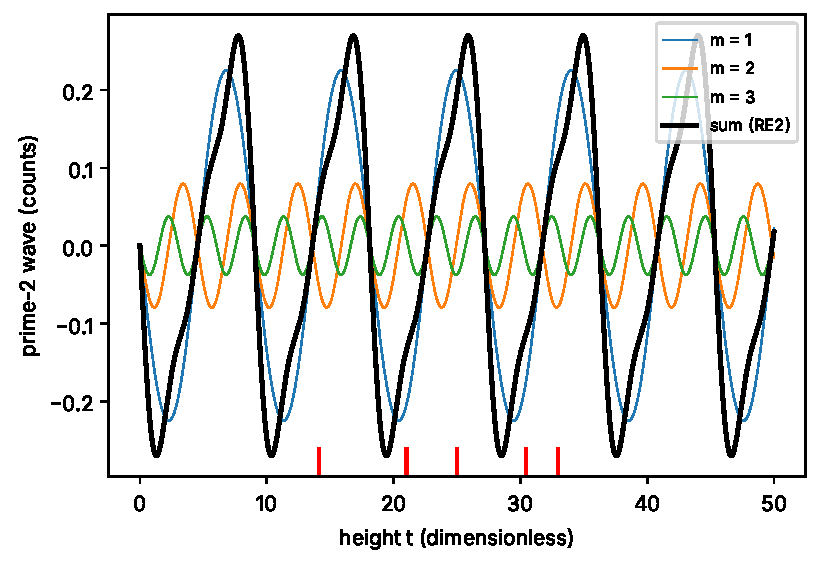
\includegraphics[width=0.85\linewidth]{figs/explicit-formula_prime2.pdf}
\caption{Running example RE2. The three harmonics $m=1,2,3$ of the prime $p=2$ (thin lines) and their sum $N^{p=2}_{\rm fl}(t)$ of \cref{eq:explicit-formula-re2} (thick line), plotted against height $t$ (dimensionless). The sum repeats with period $2\pi/\log2\approx9.065$. Vertical ticks mark the first five zeta zeros.}
\label{fig:explicit-formula-prime2}
\end{figure}

\begin{sample}{The rms size of the prime-2 wave}
Find the root mean square of $N^{p=2}_{\rm fl}(t)$ over one period.

\textbf{Step 1: mean squares of products.} Let $\omega_0=\log2$ and $T_0=2\pi/\omega_0$. By the orthogonality of sines over a period (Chapter~\ref{ch:fourier-series}),
\[
\frac{1}{T_0}\int_0^{T_0}\sin(a\omega_0t)\sin(b\omega_0t)\,\dd t=\begin{cases}\tfrac12,&a=b,\\0,&a\ne b,\end{cases}\qquad a,b\in\{1,2,3\}.
\]
\textbf{Step 2: square the sum.} Write $N^{p=2}_{\rm fl}=\sum_m c_m\sin(m\omega_0 t)$ with $c_m=-1/(\pi m2^{m/2})$. Expanding the square and averaging term by term, all cross terms vanish by Step 1, leaving
\[
\overline{\bigl(N^{p=2}_{\rm fl}\bigr)^2}=\tfrac12\sum_{m=1}^3c_m^2=\frac{1}{2\pi^2}\Bigl(\frac{1}{2}+\frac{1}{16}+\frac{1}{72}\Bigr)=\frac{0.5763889}{2\pi^2}.
\]
\textbf{Step 3: take the square root.} $\sqrt{0.5763889/2}=0.536837$, divided by $\pi$:
\[
\boxed{\rms\bigl(N^{p=2}_{\rm fl}\bigr)=0.1709.}
\]
\end{sample}

Keep this number in mind. In the paper's continuation probe (Sec.~III) the target fluctuation is exactly this wave, and the paper's App.~A lists the ``probe-null'' (the error of predicting no fluctuation on levels 401--500) as $0.1708$. Evaluating $N^{p=2}_{\rm fl}$ at the smooth zeros $s_{401},\dots,s_{500}$ and taking the rms gives the same value to within $0.003$ (verified in this chapter's check script); sampling at roughly 15 periods' worth of nearly evenly spaced points reproduces the time average.

\begin{checkpoint}
At which angular frequency does the prime power $25=5^2$ appear, what is its amplitude $1/(m\sqrt k)$, and is this wave included in the paper's Eq.~(4) when $5\in P$?
\end{checkpoint}
\checkanswer{$\omega=\log25=2\log5=3.2189$; amplitude $1/(2\cdot5)=0.1$; yes, Eq.~(4) keeps $m=1,2,3$ for every prime in $P$, so $m=2$ for $p=5$ is included.}

\begin{keyideas}
\item On a vertical line $\Re s=\sigma$, the term $p^{-ms}/m$ is a phasor of length $p^{-m\sigma}/m$ rotating at angular frequency $m\log p$ in $t$; its imaginary part is $-\sin(mt\log p)/(mp^{m\sigma})$.
\item $\Im\log\zeta(\sigma+it)$ is therefore a superposition of waves at the frequencies $\log p^m$, an almost-periodic function of $t$.
\item The prime-2 part with $m\le3$ (RE2) is periodic with period $2\pi/\log2\approx9.065$ and has rms $0.1709$ after division by $\pi$.
\end{keyideas}

%=====================================================================
\section{The formal step to the critical line}\label{sec:explicit-formula-formal}

\subsection{What we want to explain}

Recall from Chapter~\ref{ch:counting-zeros} the Riemann--von Mangoldt formula,
\begin{equation}
N(T)=\frac{\theta(T)}{\pi}+1+S(T),\qquad S(T)=\frac{1}{\pi}\arg\zeta\bigl(\tfrac12+iT\bigr),
\label{eq:explicit-formula-rvm}
\end{equation}
where $N(T)$ is the number of zeros with $0<t\le T$, $\theta$ is the Riemann--Siegel theta function, and $\theta(T)/\pi+1=\Nsm(T)+\order(1/T)$ with $\Nsm$ the smooth counting function of the paper's Eq.~(1). The argument in $S(T)$ is defined by \emph{continuous variation}: start at $s=2$, where $\zeta(2)>0$ and we take $\arg\zeta(2)=0$; move straight up to $2+iT$; then move straight left to $\tfrac12+iT$; follow the angle continuously along the way. (This works when $T$ is not the height of a zero.) So $S(T)\approx N(T)-\Nsm(T)$: the actual count minus the smooth count.

\subsection{The argument where the series converges}

For $\sigma>1$, take the imaginary part of \cref{eq:explicit-formula-logzeta} term by term using \cref{eq:explicit-formula-imterm}:
\begin{equation}
\Phi_\sigma(t)\equiv\Im\log\zeta(\sigma+it)=-\sum_p\sum_{m=1}^{\infty}\frac{\sin(mt\log p)}{m\,p^{m\sigma}} .
\label{eq:explicit-formula-phi}
\end{equation}
(Taking the imaginary part term by term is allowed because the series converges absolutely: the imaginary parts of the partial sums are the partial sums of the imaginary parts.)

Is $\Phi_\sigma(t)$ the same as the continuously varied argument used to define $S$? Three facts settle it.
\begin{enumerate}
\item $\Phi_\sigma(t)$ is \emph{an} argument of $\zeta(\sigma+it)$. Indeed, writing $\log\zeta=R+i\Phi$ with $R,\Phi$ real, $\zeta=e^{\log\zeta}=e^{R}e^{i\Phi}$, which is polar form with angle $\Phi$.
\item $\Phi_\sigma(t)$ is continuous in $\sigma$ and $t$ for $\sigma\ge\sigma_0>1$. Each term is bounded in absolute value by $p^{-m\sigma_0}/m$, a fixed summable number independent of $\sigma$ and $t$, so the convergence is uniform; a uniformly convergent series of continuous functions has a continuous sum (see the box below).
\item At $s=2$ every sine vanishes, so $\Phi_2(0)=0$, the agreed starting value.
\end{enumerate}
Two continuous arguments of the same nonvanishing function along a path differ by $2\pi\times$(an integer), and that integer, being a continuous integer-valued function, is constant. Starting from the same value $0$, they agree everywhere. So on the vertical segment from $2$ to $2+iT$, and on the horizontal segment from $2+iT$ to $\sigma+iT$ for any $\sigma>1$, the continuous argument \emph{is} $\Phi$. This much is a \textbf{theorem (proved)}.

\begin{beyond}
\textbf{Taken on trust: uniform limits are continuous.} If continuous functions $f_K$ converge to $f$ uniformly on an interval (the maximum of $\abs{f_K-f}$ tends to $0$), then $f$ is continuous. The ``M-test'' used above (if $\abs{\text{term}_j}\le M_j$ with $\sum M_j<\infty$, convergence is uniform) is its standard companion. Both are proved in any real-analysis text and in \cite{rhb}.
\end{beyond}

\subsection{The formal step}

Here is the step that is \textbf{not} justified. The path defining $S(T)$ continues from $\sigma+iT$ (with $\sigma>1$) to $\tfrac12+iT$. If we \emph{pretend} that \cref{eq:explicit-formula-phi} still holds at $\sigma=\tfrac12$ and divide by $\pi$, we obtain
\begin{equation}
S(t)\ \text{``}{=}\text{''}\ -\frac{1}{\pi}\sum_p\sum_{m=1}^{\infty}\frac{\sin(mt\log p)}{m\,p^{m/2}}
=-\frac1\pi\sum_{k=2}^{\infty}\frac{\Lambda(k)}{\sqrt{k}\,\log k}\sin(t\log k).
\qquad\text{(formal)}
\label{eq:explicit-formula-formal}
\end{equation}
The second form uses $\Lambda(k)/\log k=1/m$ and $p^{m/2}=\sqrt{k}$ for $k=p^m$. The quotation marks are deliberate. Equation~\eqref{eq:explicit-formula-formal} is a \textbf{heuristic}: it is the right \emph{shape}, and truncations of it approximate $S$ well (\cref{sec:explicit-formula-why}), but as written it is not a theorem. Three separate obstacles stand in the way.

\paragraph{Obstacle 1: no absolute convergence.} At $\sigma=\tfrac12$ the $m=1$ amplitudes are $p^{-1/2}$. We now prove that $\sum_p p^{-1/2}$ diverges, by proving the stronger fact that $\sum_p 1/p$ diverges.

\begin{sample}{The sum of the reciprocals of the primes diverges}
\textbf{Step 1: split $\log\zeta(\sigma)$ for real $\sigma>1$.} By \cref{eq:explicit-formula-logzeta},
\[
\log\zeta(\sigma)=\sum_p p^{-\sigma}+\sum_p\sum_{m\ge2}\frac{p^{-m\sigma}}{m}.
\]
\textbf{Step 2: the $m\ge2$ part is bounded.} Since $p^{-m\sigma}\le p^{-m}$ and $1/m\le1$,
\[
\sum_{m\ge2}\frac{p^{-m\sigma}}{m}\le\sum_{m\ge2}p^{-m}=\frac{p^{-2}}{1-p^{-1}}=\frac{1}{p(p-1)} .
\]
Summing over primes and then enlarging to all integers $k\ge2$,
\[
\sum_p\frac{1}{p(p-1)}\le\sum_{k=2}^{\infty}\frac{1}{k(k-1)}=\sum_{k=2}^{\infty}\Bigl(\frac{1}{k-1}-\frac1k\Bigr)=1\quad\text{(telescoping, Chapter~\ref{ch:series})}.
\]
\textbf{Step 3: $\zeta(\sigma)\to\infty$ as $\sigma\to1^+$.} Each term $k^{-\sigma}$ is at least $\int_k^{k+1}x^{-\sigma}\dd x$ because $x^{-\sigma}$ decreases, so $\zeta(\sigma)\ge\int_1^\infty x^{-\sigma}\dd x=\frac{1}{\sigma-1}$.

\textbf{Step 4: combine.} From Steps 1--3, $\sum_p p^{-\sigma}\ge\log\zeta(\sigma)-1\ge\log\frac{1}{\sigma-1}-1$, which grows without bound as $\sigma\to1^+$.

\textbf{Step 5: conclude.} For every $\sigma>1$ and every prime, $1/p\ge p^{-\sigma}$, so $\sum_p 1/p\ge\sum_p p^{-\sigma}$. The right side can be made as large as we like, hence
\[
\boxed{\sum_p\frac1p=\infty,\qquad\text{and therefore}\qquad\sum_p\frac{1}{\sqrt p}=\infty\ \ (\text{since }p^{-1/2}\ge p^{-1}).}
\]
\end{sample}

Even the $m=2$ amplitudes, $1/(2p)$, have a divergent sum by the same result. Only the $m\ge3$ terms, of size at most $p^{-3/2}/3$, converge absolutely (Problem~\ref{prob:explicit-formula-mge3}). \Cref{fig:explicit-formula-partial} shows the contrast.

\begin{figure}[htbp]\centering
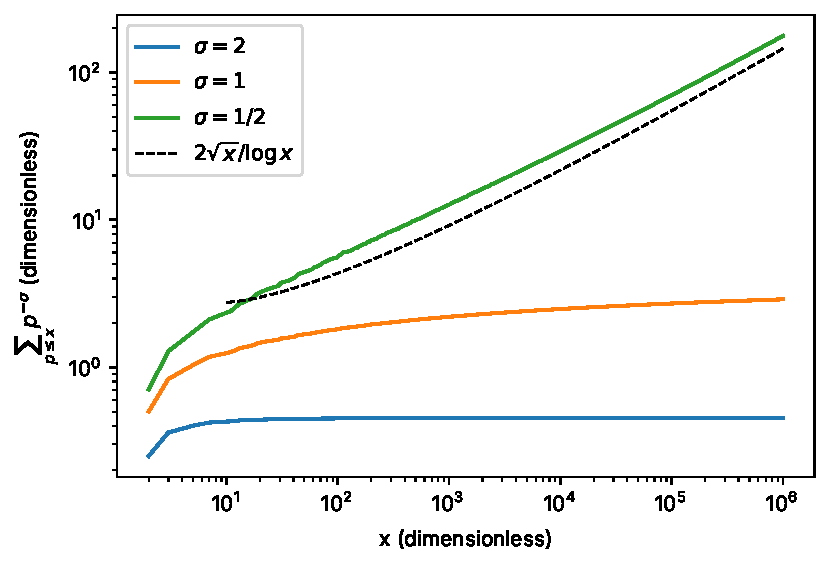
\includegraphics[width=0.85\linewidth]{figs/explicit-formula_partial.pdf}
\caption{Partial sums $\sum_{p\le x}p^{-\sigma}$ over primes up to $x$ (both axes logarithmic, dimensionless). For $\sigma=2$ the sum levels off; for $\sigma=1$ it creeps upward without bound (like $\log\log x$); for $\sigma=\tfrac12$, the critical line, it grows roughly like $\sqrt{x}$. The amplitudes of the waves in \cref{eq:explicit-formula-formal} are not summable.}
\label{fig:explicit-formula-partial}
\end{figure}

\begin{sample}{How big do the critical-line amplitudes get?}
Compute $\sum_{p\le100}p^{-1/2}$, the sum of the $m=1$ amplitudes for the 25 primes below 100 (the prime set of the paper's ``25 primes'' oracle).

\textbf{Step 1: list.} The primes are $2,3,5,\dots,97$, with $1/\sqrt p$ from $0.707107$ down to $0.101535$.

\textbf{Step 2: add} (term by term, or with \texttt{numpy}):
\[
\boxed{\sum_{p\le100}\frac{1}{\sqrt p}=5.5365.}
\]
If all 25 waves happened to peak together, the $m=1$ part alone of \cref{eq:explicit-formula-formal} would reach $5.5365/\pi\approx1.76$ (about $1.76$ mean spacings), far more than the typical size $\abs{S}<1$ found in Chapter~\ref{ch:counting-zeros}. The waves must mostly cancel.
\end{sample}

\paragraph{Obstacle 2: the strip $\tfrac12\le\sigma\le1$.} The series \cref{eq:explicit-formula-logzeta} was established only for $\sigma>1$. At $\sigma=1$ the function $\zeta$ has its pole (Chapter~\ref{ch:zeta}); our path at height $T$ avoids $s=1$, but nothing we have proved says that the series represents $\log\zeta$ anywhere with $\sigma\le1$. The value of $\arg\zeta$ on the critical line is determined by the analytic continuation of $\zeta$ (Chapter~\ref{ch:zeta}), not by the series.

\paragraph{Obstacle 3: jumps.} As $T$ passes a zero $t_n$ (assumed simple, which is verified numerically for all zeros used here), $N(T)$ jumps by $1$ while $\theta(T)$ is smooth. By \cref{eq:explicit-formula-rvm}, $S(T)$ jumps by $+1$ at every zero. Between zeros it decreases steadily, with slope $-\Nsm'(T)$ up to $\order(1/T^2)$. Every truncation of \cref{eq:explicit-formula-formal} is a finite sum of sines, hence continuous. By the box above, a sequence of continuous functions cannot converge \emph{uniformly} to a function with a jump. So no sequence of truncations can converge to $S$ uniformly on any interval containing a zero.

\begin{beyond}
\textbf{Taken on trust: rigorous versions.} (i) Everything in \cref{sec:explicit-formula-logzeta} and in \cref{eq:explicit-formula-phi} for $\sigma>1$ is proved above. (ii) Whether \cref{eq:explicit-formula-formal} converges at a given point $t$ of the critical line is not established by anything in this book, and the paper does not rely on it. (iii) What \emph{is} proved, by A.~Selberg, is that $S(t)$ is well approximated on average over $t$ by short, smoothly weighted sums over primes $p\le x$ of the form $-\frac1\pi\sum_p\sin(t\log p)/\sqrt p$, with explicit control of the error; a consequence is that $S(t)$ has mean square growing like $\frac{1}{2\pi^2}\log\log t$ and an approximately Gaussian distribution. These theorems are presented in \cite{titchmarsh}. (iv) The exact cure for the jumps is \emph{smoothing}: replace $S$ by an average of $N(t)$ against a smooth weight. Then the sum over prime powers becomes an exact identity with a convergent, smoothly cut-off prime sum: the Guinand--Weil explicit formula of \cref{sec:explicit-formula-duality}.
\end{beyond}

\begin{pitfall}
Do not write \cref{eq:explicit-formula-formal} with an equals sign and treat it as an identity. It is a formal continuation of a series that converges only for $\Re s>1$. Its truncations, used with care, are good \emph{approximations}; the paper itself presents its Eq.~(4) as a truncation used as a baseline, with ``no novelty'' and with the predictions checked against actual zeros.
\end{pitfall}

\begin{checkpoint}
The $m=3$ terms of \cref{eq:explicit-formula-formal} have amplitudes $1/(3p^{3/2})$. Does $\sum_p 1/(3p^{3/2})$ converge? What about the $m=2$ amplitudes?
\end{checkpoint}
\checkanswer{The $m=3$ sum converges: it is bounded by $\frac13\sum_{k\ge2}k^{-3/2}$, a convergent $p$-series with exponent $3/2>1$. The $m=2$ sum $\sum_p\frac{1}{2p}$ diverges, because $\sum_p 1/p$ diverges.}

\begin{keyideas}
\item For $\sigma>1$, $\Im\log\zeta(\sigma+it)=-\sum_p\sum_m\sin(mt\log p)/(mp^{m\sigma})$ exactly, and it equals the continuously varied argument.
\item Setting $\sigma=\tfrac12$ formally gives $S(t)$ ``$=$'' $-\frac1\pi\sum_p\sum_m\sin(mt\log p)/(mp^{m/2})$ (\cref{eq:explicit-formula-formal}): a heuristic, not a theorem.
\item Obstacles: the amplitudes are not summable ($\sum_p1/p=\infty$, proved), the series is not established for $\sigma\le1$, and $S$ jumps by $1$ at each zero while finite sine sums are continuous.
\item Rigorous replacements exist: Selberg's smoothed prime sums for $S(t)$, and the exact Guinand--Weil formula with smooth test functions.
\end{keyideas}

%=====================================================================
\section{Why a truncated sum still works}\label{sec:explicit-formula-why}

After the warnings of the previous section, \cref{fig:explicit-formula-staircase} may surprise you. It plots the measured $S(t)\approx N(t)-\Nsm(t)$, a sawtooth staircase, together with truncations of \cref{eq:explicit-formula-formal} keeping one prime, six primes and 25 primes (always with $m\le3$). The truncated sums are smooth, of course, but they follow the \emph{middle} of the sawtooth: wherever the jumps sit above average, the smooth curve rises; where they sit below, it falls.

\begin{figure}[htbp]\centering
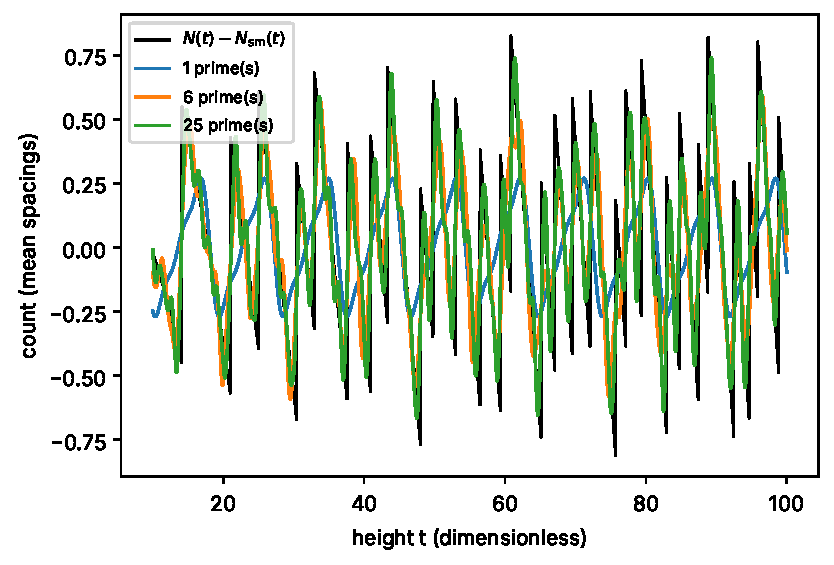
\includegraphics[width=0.85\linewidth]{figs/explicit-formula_staircase.pdf}
\caption{The measured fluctuating count $S(t)\approx N(t)-\Nsm(t)$ (black step-and-ramp curve, jumping by $+1$ at each zero) and truncations of the explicit formula with $m\le3$: primes $\{2\}$, the first 6 primes, and the first 25 primes. Horizontal axis: height $t$ (dimensionless); vertical axis: count (equivalently, mean spacings). The smooth curves follow the midpoints of the jumps.}
\label{fig:explicit-formula-staircase}
\end{figure}

\subsection{What a zero ``sees''}

At a zero, $N(t)$ jumps from $n-1$ to $n$. Adopt the convention (as in Chapter~\ref{ch:counting-zeros}) that $N(t_n)=n-\tfrac12$, the average of its left and right limits; correspondingly $S(t_n)$ means the midpoint of its jump. Then, up to the neglected $\order(1/t)$ term of $\theta/\pi$, every zero satisfies exactly
\begin{equation}
\Nsm(t_n)+S(t_n)=n-\tfrac12 .
\label{eq:explicit-formula-exactlevel}
\end{equation}
To predict $t_n$ we therefore need only the \emph{midpoint value} of $S$ at the zero, not the whole sawtooth.

\subsection{The midpoint heuristic}

Recall from Chapter~\ref{ch:fourier-series} a fact about Fourier series: for a piecewise smooth periodic function with a jump, the partial sums of its Fourier series converge at the jump to the \emph{midpoint} of the two one-sided values (with Gibbs overshoot nearby, but not at the jump itself). The prime sum \cref{eq:explicit-formula-formal} plays the role of a Fourier expansion of $S(t)$, with the prime powers as the frequencies. If the analogy holds, its truncations should approximate $S$ at a zero by the midpoint of the jump, which is exactly the quantity in \cref{eq:explicit-formula-exactlevel}.

A complementary picture: decompose $S$ into a slowly varying part and a sawtooth that jumps by $+1$ at each zero and ramps down in between. If the zeros were evenly spaced with spacing $\gap$, the sawtooth would be periodic with zero average and with its lowest frequency at $2\pi/\gap$; its midpoint value at each zero would be $0$. A sum of waves with frequencies well below $2\pi/\gap$ cannot represent the sawtooth at all; it represents only the slow part, and at a zero the slow part equals the midpoint value. With $\gap=2\pi/\log(t/2\pi)$, the condition ``well below $2\pi/\gap$'' reads $\log p^m\ll\log(t/2\pi)$. Because the real zeros are not evenly spaced, this picture is only qualitative, and including more primes than this keeps helping in practice (\cref{sec:explicit-formula-howmany}).

Status: this whole subsection is \textbf{heuristic}. The rigorous statements are those of the boxes in \cref{sec:explicit-formula-formal} and \cref{sec:explicit-formula-duality}; the practical evidence is the numerical accuracy of the resulting predictions.

\begin{sample}{The truncated formula at the first zero}
Evaluate the one-prime truncation $N^{p=2}_{\rm fl}(t)$ of \cref{eq:explicit-formula-re2} at $t=t_1=14.134725$ and compare it with $S(t_1)$ as defined by \cref{eq:explicit-formula-exactlevel}.

\textbf{Step 1: phases.} $t_1\log2=9.797442$, $2t_1\log2=19.594884$, $3t_1\log2=29.392326$. Reducing by $3\pi$, $6\pi$ and $9\pi$: $9.797442=3\pi+0.372664$, $19.594884=6\pi+0.745328$, $29.392326=9\pi+1.117992$.

\textbf{Step 2: sines.} Using $\sin(x+3\pi)=-\sin x$, $\sin(x+6\pi)=\sin x$, $\sin(x+9\pi)=-\sin x$:
\[
\sin(t_1\log2)=-0.364098,\quad\sin(2t_1\log2)=0.678213,\quad\sin(3t_1\log2)=-0.899224.
\]
\textbf{Step 3: weights.} Divide by $m2^{m/2}=1.414214,\ 4,\ 8.485281$: the three terms are $-0.257456$, $0.169553$, $-0.105975$, summing to $-0.193878$.

\textbf{Step 4: multiply by $-1/\pi$.} $N^{p=2}_{\rm fl}(t_1)=0.06171$.

\textbf{Step 5: the measured midpoint.} With $t_1/2\pi=2.2496113$ and $\log(2.2496113)=0.8107574$,
\[
\Nsm(t_1)=2.2496113\times0.8107574-2.2496113+0.875=0.44928 .
\]
So $S(t_1)=\tfrac12-0.44928=0.05072$ (neglecting corrections of order $1/t$, here $1/(48\pi t_1)\approx0.0005$).
\[
\boxed{N^{p=2}_{\rm fl}(t_1)=0.0617\quad\text{vs}\quad S(t_1)=0.0507.}
\]
A single prime gets the sign and rough size right.
\end{sample}

\begin{checkpoint}
Just below a zero, $S=-0.2$; just above it, $S=+0.8$. What value of $S$ enters \cref{eq:explicit-formula-exactlevel}, and is the zero earlier or later than the smooth zero $s_n$?
\end{checkpoint}
\checkanswer{The midpoint, $0.3$. Then $\Nsm(t_n)=n-\tfrac12-0.3<\Nsm(s_n)$, and since $\Nsm$ increases, $t_n<s_n$: the zero is early, by about $0.3$ mean spacings.}

\begin{keyideas}
\item A zero satisfies $\Nsm(t_n)+S(t_n)=n-\tfrac12$ with $S(t_n)$ the midpoint of its jump; prediction needs only that midpoint.
\item Heuristically, truncated prime sums behave like truncated Fourier series, which converge to midpoints at jumps; low frequencies carry the slow part of $S$, which is what moves zeros early or late.
\item This explanation is heuristic; its support is rigorous smoothed versions plus numerical accuracy.
\end{keyideas}

%=====================================================================
\section{Predicting the $n$-th zero}\label{sec:explicit-formula-predict}

\subsection{The level equation}

Replace the exact but unknown $S(t_n)$ in \cref{eq:explicit-formula-exactlevel} by a finite truncation. Following the paper's Eq.~(4), for a finite set of primes $P$ define
\begin{equation}
\Nfl(t)=-\frac{1}{\pi}\sum_{p\in P}\sum_{m=1}^{3}\frac{\sin(mt\log p)}{m\,p^{m/2}},
\label{eq:explicit-formula-nfl}
\end{equation}
and define the predicted $n$-th zero as the solution $t$ of
\begin{equation}
\boxed{\Nsm(t)+\Nfl(t)=n-\tfrac12 .}
\label{eq:explicit-formula-level}
\end{equation}
Two truncations are made: primes outside $P$ are dropped, and powers $m\ge4$ are dropped (their total amplitude for $p=2$ is at most $0.0487$, Problem~\ref{prob:explicit-formula-mtail}). Nothing is fitted: $P$ is chosen in advance and every coefficient is fixed by \cref{eq:explicit-formula-formal}.

\subsection{A first-order solution}

Recall from Chapter~\ref{ch:counting-zeros} that the smooth zero $s_n$ solves $\Nsm(s_n)=n-\tfrac12$, that $\Nsm'(t)=\frac{1}{2\pi}\log\frac{t}{2\pi}$, and that the mean spacing is $\gap_n=ds_n/dn=1/\Nsm'(s_n)=2\pi/\log(s_n/2\pi)$. Write the predicted zero as $t=s_n+\Delta$. Expanding to first order,
\begin{align}
\Nsm(s_n+\Delta)&\approx\Nsm(s_n)+\Nsm'(s_n)\Delta=n-\tfrac12+\frac{\Delta}{\gap_n},\label{eq:explicit-formula-lin1}\\
\Nfl(s_n+\Delta)&\approx\Nfl(s_n)+\Nfl'(s_n)\Delta.\label{eq:explicit-formula-lin2}
\end{align}
Substituting both into \cref{eq:explicit-formula-level} and cancelling $n-\tfrac12$,
\begin{equation}
\frac{\Delta}{\gap_n}+\Nfl(s_n)+\Nfl'(s_n)\Delta=0
\quad\Longrightarrow\quad
\Delta=-\frac{\Nfl(s_n)}{1/\gap_n+\Nfl'(s_n)} .
\label{eq:explicit-formula-delta}
\end{equation}
If moreover $\abs{\Nfl'}\ll1/\gap_n$ (the smooth count rises much faster than the fluctuation changes), the predicted fluctuation in mean spacings is simply
\begin{equation}
\frac{t-s_n}{\gap_n}\approx-\Nfl(s_n).
\label{eq:explicit-formula-firstorder}
\end{equation}
A positive $\Nfl$ means an early zero, as in the checkpoint above. Neglected: second-order terms in $\Delta$ (the curvature of $\Nsm$ and of $\Nfl$).

\begin{sample}{Predicting $t_1$ from the prime 2}
Predict the first zero using $P=\{2\}$, and compare with $t_1=14.134725$ and with the null prediction $s_1$.

\textbf{Step 1: the smooth zero.} Solving $\Nsm(s)=\tfrac12$ by Newton's method from $s=t_1$ (slope $0.129$, then a second iteration) gives $s_1=14.5214$, and $\gap_1=2\pi/\log(s_1/2\pi)=2\pi/0.837746=7.500$.

\textbf{Step 2: $\Nfl$ and its slope at $s_1$.} As in the previous sample, $s_1\log2=10.065465=3\pi+0.640687$, and so on; the result is $N^{p=2}_{\rm fl}(s_1)=0.09350$. Differentiating \cref{eq:explicit-formula-re2}, $\Nfl'(t)=-\frac{\log2}{\pi}\sum_{m=1}^3\frac{\cos(mt\log2)}{2^{m/2}}$, which at $s_1$ gives $\Nfl'(s_1)=0.0667$.

\textbf{Step 3: crude first order, \cref{eq:explicit-formula-firstorder}.} $t\approx s_1-\gap_1\Nfl(s_1)=14.5214-0.7012=13.820$. This overshoots badly.

\textbf{Step 4: why, and the better first order.} At $t\approx14$, $1/\gap_1=0.1333$ while $\Nfl'(s_1)=0.0667$: the condition $\abs{\Nfl'}\ll1/\gap$ fails. Using \cref{eq:explicit-formula-delta}, $\Delta=-0.09350/(0.13333+0.06675)=-0.4673$, so $t\approx14.054$.

\textbf{Step 5: solve \cref{eq:explicit-formula-level} exactly.} Let $f(t)=\Nsm(t)+\Nfl(t)-\tfrac12$. Evaluating, $f(13.8202)=-0.0635$ and $f(14.1347)=+0.0110$: a sign change, so a root lies between (bisection logic, Chapter~\ref{ch:asymptotics}). Linear interpolation gives $14.0883$, where $f=+0.00036$; one more secant step gives the root
\[
\boxed{t^{\rm pred}_1=14.087.}
\]
\textbf{Step 6: compare in mean spacings.} True fluctuation $(t_1-s_1)/\gap_1=-0.0516$; predicted $(14.087-14.5214)/7.500=-0.0580$; null $0$. The prediction error is $0.0064$ spacings against the null's $0.0516$.
\end{sample}

\subsection{How many roots?}

\Cref{eq:explicit-formula-level} asks where the increasing function $\Nsm$ plus a wiggle crosses a horizontal line. If the wiggle's slope can be more negative than the rise of $\Nsm$, the sum can turn down and cross the same line two or three times (\cref{fig:explicit-formula-levelfn}). A safe condition for a single crossing is that $\Nsm'(t)+\Nfl'(t)>0$ everywhere near the crossing.

\begin{sample}{When is the prime-2 root unique?}
Find a height above which the level equation with $P=\{2\}$ has at most one root.

\textbf{Step 1: bound the wiggle's slope.} Differentiating \cref{eq:explicit-formula-re2} and using $\abs{\cos}\le1$,
\[
\abs{\Nfl'(t)}\le\frac{\log2}{\pi}\Bigl(\frac{1}{\sqrt2}+\frac12+\frac{1}{2\sqrt2}\Bigr)=\frac{0.693147\times1.560660}{\pi}=0.34434 .
\]
\textbf{Step 2: compare with the smooth slope.} $\Nsm'(t)=\frac{1}{2\pi}\log\frac{t}{2\pi}$ exceeds $0.34434$ when $\log\frac{t}{2\pi}>2\pi\times0.34434=2.16353$, i.e.\ $\frac{t}{2\pi}>e^{2.16353}=8.7018$.

\textbf{Step 3: conclude.} For $t>2\pi\times8.7018$, the function $\Nsm+\Nfl$ is strictly increasing, so it crosses each level $n-\tfrac12$ at most once:
\[
\boxed{t>54.7\ \Rightarrow\ \text{unique root for }P=\{2\}.}
\]
Below $54.7$ uniqueness is not guaranteed by this bound (although in the previous sample the root near $14$ was unique within the bracket used). With more primes the bound on $\abs{\Nfl'}$ grows, so the guaranteed height rises; for $P=\{2,3\}$ it is about $617$ (Problem~\ref{prob:explicit-formula-unique23}). The bound is a worst case: all waves would have to reach their steepest descent simultaneously.
\end{sample}

\begin{figure}[htbp]\centering
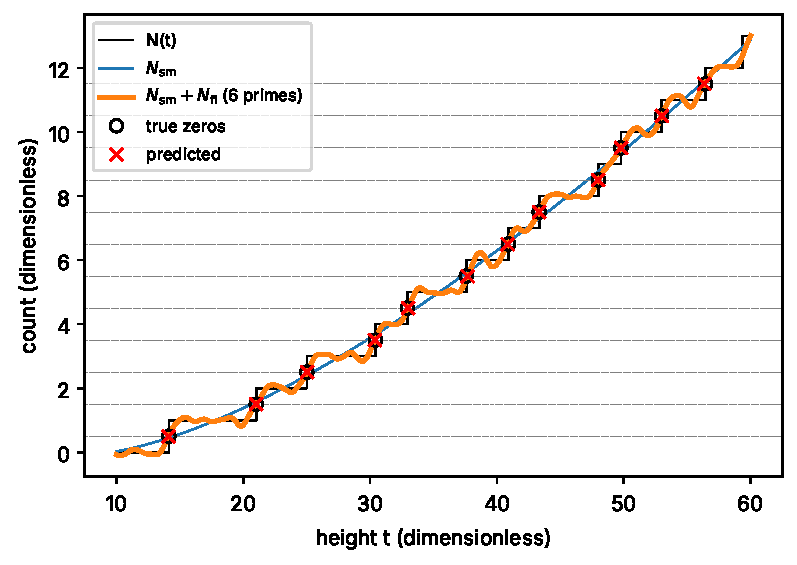
\includegraphics[width=0.85\linewidth]{figs/explicit-formula_levelfn.pdf}
\caption{The level equation. Staircase: the true count $N(t)$. Thin smooth line: $\Nsm(t)$. Thick line: $\Nsm(t)+\Nfl(t)$ with the first six primes. Dashed horizontal lines: the levels $n-\tfrac12$. Open circles: true zeros; crosses: predicted zeros (roots of \cref{eq:explicit-formula-level}). Horizontal axis height $t$, vertical axis count (dimensionless).}
\label{fig:explicit-formula-levelfn}
\end{figure}

\begin{pitfall}
When $\Nfl$ has large amplitude or contains steep high-frequency terms, \cref{eq:explicit-formula-level} can have several roots near $s_n$. A root finder then returns \emph{one} of them, determined by the bracket, and the ``prediction'' depends on that arbitrary choice. Always check for multiple roots. The paper flags exactly this for one of its fitted controls (Sec.~IV): the level equation ``has several roots for about a third of the held-out levels''.
\end{pitfall}

\subsection{The paper's procedure}

The paper's App.~A, step (8), solves \cref{eq:explicit-formula-level} with Brent's method (Chapter~\ref{ch:asymptotics}) bracketed by $\pm3$ mean spacings around $s_n$, with the bracket expanded if the function does not change sign at its ends. Here is the same procedure in a few lines.

\begin{pycode}
import numpy as np, qmnt
from scipy.optimize import brentq

P = qmnt.first_primes(6)                    # 2, 3, 5, 7, 11, 13

def level_fn(t, n):
    """N_sm(t) + N_fl(t) - (n - 1/2): its root is the predicted zero."""
    return qmnt.Nsm(t) + qmnt.Nfl(t, P, mmax=3) - (n - 0.5)

n = 450
s = brentq(lambda t: qmnt.Nsm(t) - (n - 0.5), 10.0, 5000.0)   # smooth zero
g = 2*np.pi/np.log(s/(2*np.pi))                             # mean gap
a, b = s - 3*g, s + 3*g                     # bracket +-3 gaps (App. A step 8)
while level_fn(a, n)*level_fn(b, n) > 0:     # expand on sign failure
    a, b = a - g, b + g
t_pred = brentq(level_fn, a, b, args=(n,))
t_true = qmnt.zeros(n)[-1]
print("predicted fluctuation", (t_pred - s)/g)
print("true fluctuation     ", (t_true - s)/g)
\end{pycode}

\subsection{The Fran\c{c}a--LeClair form and Lambert's $W$}

Fran\c{c}a and LeClair \cite{francaleclair,leclair} wrote the exact condition \cref{eq:explicit-formula-exactlevel} as a transcendental equation for the $n$-th zero. Since $\Nsm(t)=\frac{t}{2\pi}\log\frac{t}{2\pi e}+\frac78$, it reads
\begin{equation}
\frac{t_n}{2\pi}\log\frac{t_n}{2\pi e}+S(t_n)=n-\frac{11}{8},
\label{eq:explicit-formula-fl}
\end{equation}
where $S(t_n)$ is understood as the appropriate limit at the zero (they take a limit from slightly off the critical line). Drop $S$ and solve the smooth part exactly. Put $A=n-\frac{11}{8}$ and $y=t/(2\pi e)$, so that $\frac{t}{2\pi}=ey$ and the equation becomes $e\,y\log y=A$. Put $y=e^{u}$:
\[
u\,e^{u}=\frac{A}{e}\quad\Longrightarrow\quad u=W\!\left(\frac Ae\right),
\]
where $W$ is Lambert's function, defined by $W(z)e^{W(z)}=z$ (Chapter~\ref{ch:asymptotics}). Then $y=e^{u}=\frac{A/e}{W(A/e)}$ (because $e^{W(z)}=z/W(z)$), and
\begin{equation}
s_n=2\pi e\,y=\frac{2\pi\,(n-\tfrac{11}{8})}{W\!\left((n-\tfrac{11}{8})/e\right)} .
\label{eq:explicit-formula-lambert}
\end{equation}
For $n=1$, $A=-\tfrac38$ and $W(-0.13795)=-0.16226$ on the principal branch, giving $s_1=14.521$, in agreement with the Newton value above. This is the ``Lambert-$W$ asymptotic of the counting function'' mentioned in the paper's Sec.~I~A. The prime corrections of Fran\c{c}a and LeClair are truncations of the classical explicit formula, the same idea as \cref{eq:explicit-formula-level}.

\begin{checkpoint}
Why does the paper bracket the root around $s_n$ rather than, say, around $s_{n+1}$?
\end{checkpoint}
\checkanswer{Because $\abs{\Nfl}$ is typically well below one count, the predicted zero lies within a fraction of a spacing of $s_n$ (\cref{eq:explicit-formula-firstorder}); a bracket of $\pm3$ spacings around $s_n$ is wide enough to contain it and narrow enough not to reach the root belonging to level $n\pm3$ or beyond.}

\begin{keyideas}
\item The predicted $n$-th zero solves $\Nsm(t)+\Nfl(t)=n-\tfrac12$ (\cref{eq:explicit-formula-level}), with zero fitted parameters.
\item To first order, the predicted fluctuation in mean spacings is $-\Nfl(s_n)$, valid when $\abs{\Nfl'}\ll1/\gap_n$; otherwise use \cref{eq:explicit-formula-delta} or solve exactly.
\item The root is unique where $\Nsm'+\Nfl'>0$; for $P=\{2\}$ this is guaranteed above $t\approx54.7$. Large or steep corrections create root ambiguity.
\item Dropping $S$ gives the smooth zeros in closed form, $s_n=2\pi(n-\frac{11}{8})/W((n-\frac{11}{8})/e)$.
\end{keyideas}

%=====================================================================
\section{How many primes?}\label{sec:explicit-formula-howmany}

\subsection{Scoring a prediction}

Recall the paper's scoring (Chapter~\ref{ch:counting-zeros}): for each held-out index $n$, convert both the true and the predicted zero into fluctuations in mean spacings, $(t_n-s_n)/\gap_n$ and $(t^{\rm pred}_n-s_n)/\gap_n$. Report the \textbf{rms} of their difference and the Pearson \textbf{correlation} (``corr'') between them. The \textbf{null} predicts $t^{\rm pred}_n=s_n$, so its rms is the rms of the true fluctuations; on zeros 401--500 (running example RE5) it is $0.263$.

\subsection{Accuracy versus the prime budget}

\Cref{tab:explicit-formula-tableV} reproduces the first two rows of the paper's Table~V. Every entry was recomputed with \texttt{qmnt.oracle\_zeros} and \texttt{qmnt.score} and agrees with the paper to the digits shown (this chapter's check script asserts this).

\begin{table}[htbp]\centering
\caption{Accuracy of the truncated explicit formula (rms in mean spacings / corr), zero fitted parameters, $m\le3$. Quoted from the paper's Table~V and reproduced with \texttt{qmnt}. ``6 primes'' means $P=\{2,3,5,7,11,13\}$; ``25 primes'' means all primes below 100.}
\label{tab:explicit-formula-tableV}
\begin{tabular}{lccccc}
\toprule
holdout & null & $\{2\}$ & 3 primes & 6 primes & 25 primes\\
\midrule
401--500 & 0.263 & 0.198 / $+0.66$ & 0.116 / $+0.90$ & 0.074 / $+0.96$ & 0.043 / $+0.99$\\
501--1000 & 0.270 & 0.208 / $+0.64$ & 0.127 / $+0.88$ & 0.083 / $+0.95$ & 0.050 / $+0.99$\\
\bottomrule
\end{tabular}
\end{table}

\begin{pycode}
import numpy as np, qmnt

n = np.arange(401, 501)                       # RE5, the principal holdout
z = qmnt.zeros(500)
print("null rms", qmnt.rms(qmnt.fluct(z[n-1], n)))   # about 0.263

for k in [1, 3, 6, 25]:
    P = qmnt.first_primes(k)
    t_pred = qmnt.oracle_zeros(n, P, mmax=3)   # roots of N_sm + N_fl = n - 1/2
    r, c = qmnt.score(t_pred, n)               # rms and corr in mean spacings
    print(f"{k:2d} primes: rms {r:.3f}  corr {c:+.2f}")
\end{pycode}

\Cref{fig:explicit-formula-holdout} shows the six-prime predictions against the truth on zeros 401--500 and the rms error as a function of the number of primes. Three features stand out.
\begin{enumerate}
\item \textbf{One prime already helps.} With $P=\{2\}$ the error drops from $0.263$ to $0.198$ and the correlation is $+0.66$: the prime-2 wave alone carries a real share of the fluctuation.
\item \textbf{Slow, steady improvement.} The amplitudes decay only like $1/\sqrt p$ (\cref{sec:explicit-formula-formal}), so each additional prime contributes a little; the error falls gradually rather than collapsing.
\item \textbf{Height independence.} Going from zeros 401--500 to 501--1000, both the null and the oracle errors grow slightly, but the ratio barely changes. The paper's Table~V continues this through zero $10^4$.
\end{enumerate}

\begin{figure}[htbp]\centering
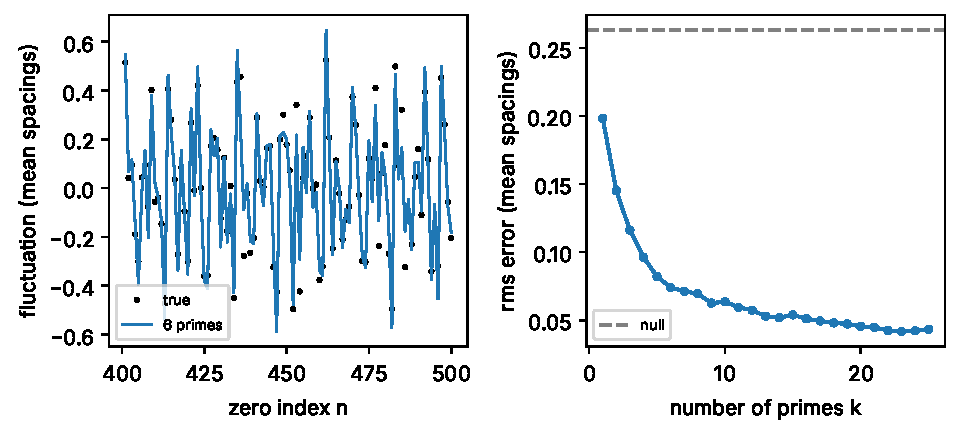
\includegraphics[width=0.95\linewidth]{figs/explicit-formula_holdout.pdf}
\caption{Left: true fluctuations $(t_n-s_n)/\gap_n$ of zeros 401--500 (dots) and the six-prime prediction (line), both in mean spacings, against the zero index $n$. Right: rms error on zeros 401--500 against the number of primes in $P$ (the first $k$ primes, $m\le3$); dashed line: the null.}
\label{fig:explicit-formula-holdout}
\end{figure}

\begin{checkpoint}
Two predictors on the same holdout have corr $+0.66$ and $+0.96$. Which can you say is more accurate in rms without further information, and why might a predictor with high corr still have a large rms?
\end{checkpoint}
\checkanswer{Neither statement follows from correlation alone (Chapter~\ref{ch:probability}): correlation measures shape, not amplitude. A predictor with the right shape but twice the true amplitude, or a constant offset, has high corr and large rms. In Table~V both metrics improve together, so there the six-prime row is better on both counts.}

\begin{keyideas}
\item Scores are rms and corr of predicted vs true fluctuations in mean spacings, relative to the null ($0.263$ on zeros 401--500).
\item With zero fitted parameters, the truncated formula gives $0.198/+0.66$ (one prime), $0.074/+0.96$ (six primes), $0.043/+0.99$ (25 primes) on zeros 401--500; qmnt reproduces these.
\item Improvement with more primes is gradual, reflecting the slow $1/\sqrt p$ decay of the amplitudes, and nearly independent of height.
\end{keyideas}

%=====================================================================
\section{The explicit formula as a duality}\label{sec:explicit-formula-duality}

Equation~\eqref{eq:explicit-formula-formal} says that the prime powers are the \emph{frequencies} of the zeros' fluctuations. Riemann's 1859 memoir \cite{riemann1859} (see \cite{edwards} for a guided reading) already contained the mirror statement: the zeros are the frequencies of the primes' fluctuations. Both are faces of one exact identity.

\subsection{The primes, built from the zeros}

Recall Chebyshev's function $\psi(x)=\sum_{k\le x}\Lambda(k)$ from Chapter~\ref{ch:primes}: a staircase that jumps by $\log p$ at each prime power $p^m$, and grows like $x$ by the prime number theorem. Let $\psi_0(x)$ be the same staircase with the value at each jump replaced by the midpoint.

\begin{beyond}
\textbf{The Riemann--von Mangoldt explicit formula (proved; proof beyond this book).} For $x>1$,
\begin{equation}
\psi_0(x)=x-\sum_{\rho}\frac{x^{\rho}}{\rho}-\log(2\pi)-\tfrac12\log\bigl(1-x^{-2}\bigr),
\label{eq:explicit-formula-psi}
\end{equation}
where the sum runs over all nontrivial zeros $\rho$, taken in symmetric pairs $\rho,\bar\rho$ in order of increasing $\abs{\Im\rho}$. The sum converges (conditionally) for each $x$. A proof is given in \cite{davenport}; see also \cite{edwards}.
\end{beyond}

Pair each zero $\rho_n=\tfrac12+it_n$ with its mirror image $\bar\rho_n$. Since $x^{\bar\rho}/\bar\rho$ is the complex conjugate of $x^{\rho}/\rho$, the pair contributes $2\Re(x^{\rho_n}/\rho_n)$. Using $x^{\rho_n}=x^{1/2}e^{it_n\log x}$,
\begin{equation}
-2\Re\frac{x^{\rho_n}}{\rho_n}=-\frac{2\sqrt x}{\abs{\rho_n}}\cos\bigl(t_n\log x-\arg\rho_n\bigr).
\label{eq:explicit-formula-psiwave}
\end{equation}
As a function of $\log x$, each zero contributes a wave of angular frequency $t_n$ and amplitude $2\sqrt x/\abs{\rho_n}$. Compare: in \cref{eq:explicit-formula-formal}, each prime power contributes a wave in $t$ of angular frequency $\log p^m$. The roles of ``position'' and ``frequency'' are swapped. \Cref{fig:explicit-formula-psi} shows how adding more zero-waves sharpens the prime staircase.

\begin{figure}[htbp]\centering
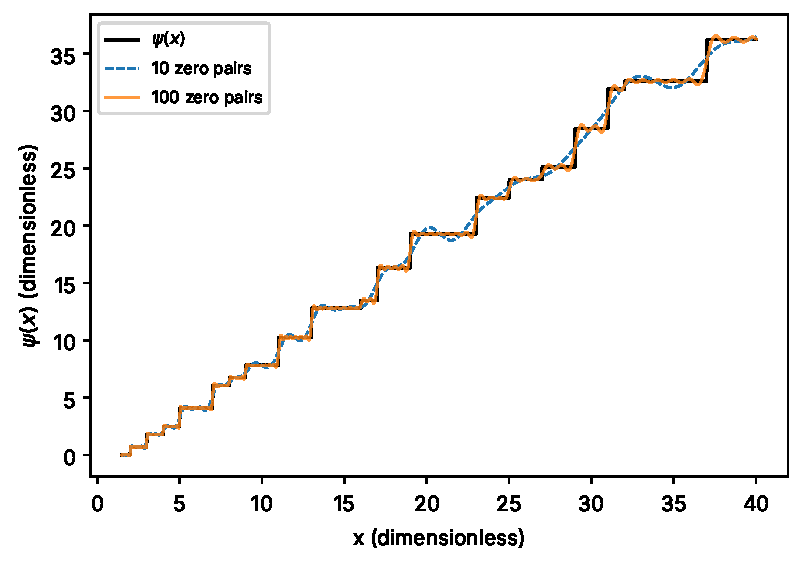
\includegraphics[width=0.85\linewidth]{figs/explicit-formula_psi.pdf}
\caption{The primes from the zeros. Staircase: $\psi(x)$, jumping by $\log p$ at each prime power. Smooth curves: the right side of \cref{eq:explicit-formula-psi} truncated to the first 10 and first 100 pairs of zeros. Horizontal axis $x$, vertical axis $\psi$ (both dimensionless).}
\label{fig:explicit-formula-psi}
\end{figure}

\begin{sample}{The size of the first zero's wave in $\psi(x)$}
Find the amplitude $2\sqrt x/\abs{\rho_1}$ of the first zero pair's wave at $x=10$ and at $x=100$.

\textbf{Step 1: $\abs{\rho_1}$.} $\abs{\rho_1}^2=\tfrac14+t_1^2=0.25+199.790451=200.040451$, so $\abs{\rho_1}=14.143566$.

\textbf{Step 2: $x=10$.} $2\sqrt{10}=6.324555$, divided by $14.143566$: $0.4472$.

\textbf{Step 3: $x=100$.} $2\times10/14.143566=1.4141$.
\[
\boxed{0.4472\ \text{at}\ x=10,\qquad 1.4141\ \text{at}\ x=100.}
\]
The waves grow like $\sqrt x$, while $\psi(x)$ itself grows like $x$; relative to $\psi$, the zero-waves shrink like $1/\sqrt x$. This $\sqrt x$ is the $\Re\rho=\tfrac12$ of the critical line made visible: a zero off the line, with $\Re\rho=\beta>\tfrac12$, would produce a wave growing like $x^{\beta}$.
\end{sample}

\subsection{The Guinand--Weil form}

The formula \cref{eq:explicit-formula-psi} sums a smooth function of the zeros (the waves) to produce a jumpy function of $x$. Its mirror version sums a function of the zeros to produce prime terms, and it becomes an exact, absolutely convergent identity once both sides are smoothed.

\begin{beyond}
\textbf{The Guinand--Weil explicit formula (proved; proof beyond this book).} Let $h(r)$ be an even function that extends analytically to the strip $\abs{\Im r}\le\tfrac12+\epsilon$ and decays fast enough there, and let $g(u)=\frac{1}{2\pi}\int_{-\infty}^{\infty}h(r)e^{-iru}\dd r$ be its Fourier transform. Write each nontrivial zero as $\rho=\tfrac12+i\gamma$ (with $\gamma=\pm t_n$ for zeros on the critical line). Then, in one common normalization,
\begin{equation}
\sum_{\rho}h(\gamma)=h\bigl(\tfrac{i}{2}\bigr)+h\bigl(-\tfrac{i}{2}\bigr)-g(0)\log\pi+\frac{1}{2\pi}\int_{-\infty}^{\infty}h(r)\,\Re\frac{\Gamma'}{\Gamma}\Bigl(\frac14+\frac{ir}{2}\Bigr)\dd r-2\sum_{k=2}^{\infty}\frac{\Lambda(k)}{\sqrt k}\,g(\log k).
\label{eq:explicit-formula-weil}
\end{equation}
The left side is a sum over zeros; the last term is a sum over prime powers. Proofs appear, in varying normalizations, in advanced texts on analytic number theory; the special case \cref{eq:explicit-formula-psi} is proved in \cite{davenport}.
\end{beyond}

Read \cref{eq:explicit-formula-weil} as a duality: probe the zeros with a function $h$, and the primes respond through its Fourier transform $g$, evaluated at the frequencies $\log k$. A smooth $h$ has a rapidly decaying $g$, so the prime sum effectively stops at some finite $k$: this is the exact version of ``truncating the prime sum''.

\paragraph{A formal check: recovering $N(T)$.} Choose $h$ to be the box: $h(r)=1$ for $\abs r\le T$, $0$ otherwise. This $h$ is not smooth, so the following is \textbf{formal}, but it shows where \cref{eq:explicit-formula-formal} comes from.
\begin{enumerate}
\item \emph{Left side.} Zeros come in pairs $\pm t_n$, so $\sum_\rho h(\gamma)=2N(T)$.
\item \emph{Transform.} $g(u)=\frac{1}{2\pi}\int_{-T}^{T}e^{-iru}\dd r=\frac{1}{2\pi}\cdot\frac{2\sin(Tu)}{u}=\frac{\sin(Tu)}{\pi u}$, and $g(0)=T/\pi$ (the limit $u\to0$).
\item \emph{Gamma term.} By Stirling's formula for complex arguments (Chapter~\ref{ch:asymptotics}), $\frac{\Gamma'}{\Gamma}(z)\approx\log z$ for large $\abs z$, so $\Re\frac{\Gamma'}{\Gamma}(\frac14+\frac{ir}{2})\approx\log\abs{\tfrac14+\tfrac{ir}2}\approx\log\frac{\abs r}{2}$. Hence the integral is approximately $\frac{1}{2\pi}\cdot2\int_0^T\log\frac r2\,\dd r=\frac1\pi\bigl[T\log\frac T2-T\bigr]$, using $\int\log\frac r2\,\dd r=r\log\frac r2-r$.
\item \emph{Constant terms.} Combining $-g(0)\log\pi=-\frac{T}{\pi}\log\pi$ with step 3 gives $\frac T\pi\bigl(\log\frac{T}{2\pi}-1\bigr)$. The terms $h(\pm\frac i2)$ and the corrections to Stirling contribute amounts that do not grow with $T$ (in a careful treatment they produce the $\frac78$ of Chapter~\ref{ch:counting-zeros}); we do not track them here.
\item \emph{Prime term.} $-2\sum_k\frac{\Lambda(k)}{\sqrt k}\frac{\sin(T\log k)}{\pi\log k}$.
\item \emph{Divide by 2.}
\[
N(T)\approx\frac{T}{2\pi}\log\frac{T}{2\pi}-\frac{T}{2\pi}+(\text{const})-\frac{1}{\pi}\sum_{k}\frac{\Lambda(k)}{\sqrt k\log k}\sin(T\log k).
\]
\end{enumerate}
The first two terms are $\Nsm(T)$ without its constant, and the last is exactly the formal series \cref{eq:explicit-formula-formal}. The non-smooth box is precisely what makes the prime sum fail to converge absolutely; smoothing $h$ repairs it.

\subsection{Landau's formula: the spectrum of the zeros}

Now probe the zeros with a pure wave: compute $\sum_n x^{\rho_n}$ over the zeros up to height $T$. If the zeros were randomly placed, this would be a random walk of size about $\sqrt{N(T)}$. Landau proved that it is not.

\begin{beyond}
\textbf{Landau's formula (proved; proof beyond this book).} For fixed $x>1$, as $T\to\infty$,
\begin{equation}
\sum_{0<t_n\le T}x^{\rho_n}=-\frac{T}{2\pi}\Lambda(x)+\order(\log T),
\label{eq:explicit-formula-landau}
\end{equation}
where $\Lambda(x)=0$ unless $x$ is an integer prime power \cite{landau}. A version uniform in $x$ is due to Gonek \cite{gonek}.
\end{beyond}

Write $x=e^{\omega}$. Then $x^{\rho_n}=e^{\omega/2}e^{i\omega t_n}$, and the real part of \cref{eq:explicit-formula-landau} gives
\begin{equation}
\sum_{0<t_n\le T}\cos(\omega t_n)\approx-\frac{T}{2\pi}\frac{\Lambda(e^{\omega})}{e^{\omega/2}}.
\label{eq:explicit-formula-landaucos}
\end{equation}
The left side is the (cosine) Fourier transform of the set of zeros, viewed as a comb of spikes at the heights $t_n$ (Chapter~\ref{ch:fourier-transform}). The right side is zero except at $\omega=\log p^m$, where it is a large negative spike growing linearly with $T$. So \emph{the spectrum of the zeros consists of lines at the logarithms of prime powers}. With a finite window the lines have width about $2\pi/T$, the resolution of Chapter~\ref{ch:fourier-transform}.

\begin{sample}{Predicted spectral lines for the first 1000 zeros}
Using \cref{eq:explicit-formula-landaucos} with $T=t_{1000}=1419.42248$, predict $\sum_{n\le1000}\cos(\omega t_n)$ at $\omega=\log2$, $\log3$ and $\log4$.

\textbf{Step 1: the common factor.} $T/2\pi=225.908$.

\textbf{Step 2: the weights $\Lambda(k)/\sqrt k$.} $k=2$: $0.693147/1.414214=0.490129$. $k=3$: $1.098612/1.732051=0.634285$. $k=4$: $\Lambda(4)=\log2$, so $0.693147/2=0.346574$.

\textbf{Step 3: multiply.}
\[
\boxed{\sum\cos(\omega t_n)\approx-110.7\ (\omega=\log2),\quad-143.3\ (\log3),\quad-78.3\ (\log4).}
\]
These are predictions; the computed sum, plotted in \cref{fig:explicit-formula-landau}, shows dips of this size at these frequencies (the error term is of order $\log T\approx7$). Notice that the line at $\log3$ is deeper than the line at $\log2$: the weight $\log p/\sqrt p$ is largest near $p=7$ (Problem~\ref{prob:explicit-formula-landau57}).
\end{sample}

\begin{figure}[htbp]\centering
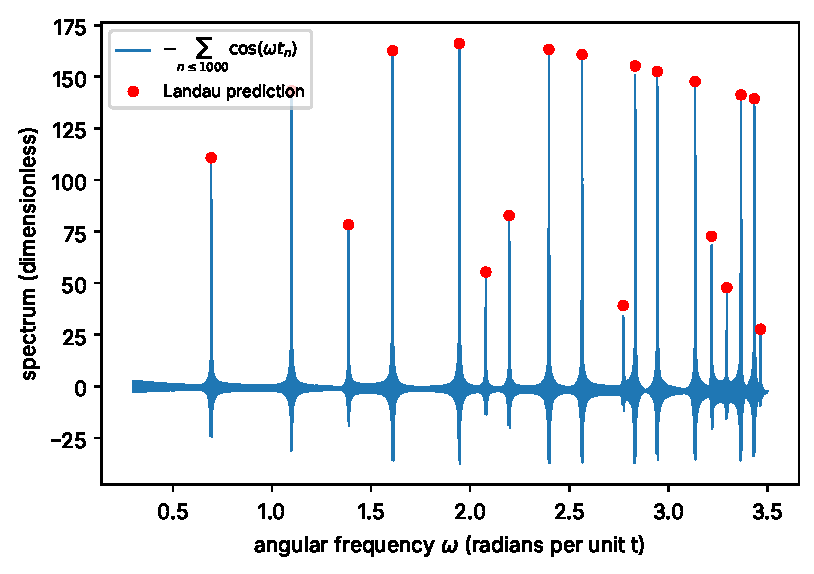
\includegraphics[width=0.85\linewidth]{figs/explicit-formula_landau.pdf}
\caption{The spectrum of the zeros. Line: $-\sum_{n\le1000}\cos(\omega t_n)$ against angular frequency $\omega$ (radians per unit $t$). Dots: Landau's prediction $\frac{T}{2\pi}\Lambda(e^\omega)e^{-\omega/2}$ at each prime power $e^{\omega}=p^m$, with $T=t_{1000}$. The peaks sit at $\log2,\log3,\log4,\log5,\log7,\dots$.}
\label{fig:explicit-formula-landau}
\end{figure}

\begin{pycode}
import numpy as np, qmnt

t = qmnt.zeros(1000)                    # heights t_1 ... t_1000
T = t[-1]
omega = np.linspace(0.3, 3.5, 6401)     # step 5e-4, finer than 2*pi/T
spec = -np.array([np.cos(w*t).sum() for w in omega])
for k, lab in [(2, "log 2"), (3, "log 3"), (4, "log 4")]:
    i = np.argmin(abs(omega - np.log(k)))
    lam = np.log(2) if k in (2, 4) else np.log(3)
    print(lab, spec[i], "Landau:", T/(2*np.pi)*lam/np.sqrt(k))
\end{pycode}

This is the fact that the paper's sparse control C2 uses without being told: a model that only assumes ``a few sinusoids in $t$'' and looks for the largest periodogram peaks of the zeros' fluctuations finds frequencies at $\log p^m$ (Chapter~\ref{ch:sparse-frequency}).

\subsection{How far can prime-only constructions go?}

Our truncation \cref{eq:explicit-formula-level} is deliberately simple. Much more refined prime-only constructions exist. As the paper reports (Sec.~I~A, paragraph b), Connes \cite{connes26} extremizes a truncated form of Weil's quadratic form built from the primes $p\le13$ and obtains approximations to the first 50 zeros with accuracies from $10^{-3}$ down to $2.6\times10^{-55}$, provably on the critical line. We mention this only to locate our baseline: the paper uses the simple truncation as an ``information-existence baseline'', not as the best possible arithmetic predictor.

\begin{checkpoint}
In \cref{eq:explicit-formula-psiwave} the angular frequency (in $\log x$) of the $n$-th wave is $t_n$; in \cref{eq:explicit-formula-formal} the angular frequency (in $t$) of the $p^m$ wave is $\log p^m$. What plays the role of the amplitude in each?
\end{checkpoint}
\checkanswer{In $\psi(x)$: $2\sqrt x/\abs{\rho_n}$, decreasing like $1/t_n$ for high zeros. In $S(t)$: $1/(\pi m p^{m/2})$, decreasing like $1/\sqrt{p^m}$ for large prime powers.}

\begin{keyideas}
\item The explicit formula is an exact duality: $\psi_0(x)=x-\sum_\rho x^\rho/\rho-\log2\pi-\frac12\log(1-x^{-2})$ builds the primes from waves with frequencies $t_n$ (in $\log x$).
\item The Guinand--Weil formula, \cref{eq:explicit-formula-weil}, relates sums over zeros of a smooth $h$ to sums over prime powers of its transform $g(\log k)$; a sharp cutoff formally reproduces $N(T)\approx\Nsm(T)+$ the formal series.
\item Landau's formula: $\sum_{t_n\le T}x^{\rho_n}\approx-\frac{T}{2\pi}\Lambda(x)$, so the Fourier spectrum of the zeros has lines at $\log p^m$ of depth $\frac{T}{2\pi}\Lambda(p^m)/p^{m/2}$.
\item Far more accurate prime-only constructions exist (Connes, first 50 zeros); the simple truncation is a baseline.
\end{keyideas}

%=====================================================================
\section{Paper connection}\label{sec:explicit-formula-paper}

\paragraph{Eq.~(4) is \cref{eq:explicit-formula-nfl}.} The paper's arithmetic oracle (Sec.~II~D) is the truncation of the formal series \cref{eq:explicit-formula-formal} to a prime set $P$ with $m\le3$, and its predicted zeros solve $\Nsm(t)+\Nfl(t)=n-\tfrac12$, our \cref{eq:explicit-formula-level}. The paper is explicit that the formula ``has no fitted parameters and no novelty'' and cites Fran\c{c}a and LeClair \cite{francaleclair,leclair}; Sec.~I~A~(b) adds that these are ``truncations of the classical Riemann--von Mangoldt/Guinand--Weil explicit formula'' (our \cref{sec:explicit-formula-duality}) and that ``the Lambert-$W$ asymptotic of the counting function'' is the smooth part (our \cref{eq:explicit-formula-lambert}). The paper also stresses that the oracle ``is not a fair ML competitor (it encodes the known functional form)'': its role is to show that predictive information exists.

\paragraph{App.~A step (8): how the roots are found.} ``Eq.~(4), $m\le3$, Brent bracketed $\pm3$ around the smooth zero (bracket expanded on sign failure).'' That is the procedure of our listing in \cref{sec:explicit-formula-predict}; the uniqueness discussion there explains why a bracket must be chosen with care.

\paragraph{Table~V.} Each column is \cref{eq:explicit-formula-level} with a different $P$: $\{2\}$, the first 3, 6, and 25 primes. The rows 401--500 and 501--1000 are reproduced in our \cref{tab:explicit-formula-tableV}. The paper's caption notes that ``the mild growth at fixed prime budget mirrors the growth of the null'', which grows from $0.263$ to $0.296$ over the table, and that ``relative skill is nearly constant''; the six-prime correlation intervals are $[+0.95,+0.97]$ on 401--500 and $[+0.91,+0.92]$ on 5001--10000.

\paragraph{Fig.~1.} The right-hand curve (``six-prime explicit formula'') is the left panel of our \cref{fig:explicit-formula-holdout}, extended into the training region; its held-out correlation $+0.96$ matches Table~V. The fitted operator's held-out correlation in the same figure is $-0.07$ (Chapters~\ref{ch:paper-memorization} and \ref{ch:generalization}).

\paragraph{Sec.~IV and Table~IV, controls A and B.} Control A is \cref{eq:explicit-formula-level} with up to 300 primes (900 terms), still with nothing fitted; it reaches $0.018$ on zeros 401--500, continuing the slow improvement of our \cref{fig:explicit-formula-holdout}. Control B keeps the frequencies $m\log p$ of \cref{eq:explicit-formula-nfl} but fits the amplitudes; with 25 primes (150 coefficients) it gives $0.028$. With 150 primes (900 coefficients on 400 zeros) it degrades to $0.180$ and is flagged root-ambiguous: the level equation ``has several roots for about a third of the held-out levels'' and ``the score varies by at most $0.012$ with the choice of root''. This is the multiple-root situation of our \cref{fig:explicit-formula-levelfn} and pitfall: fitted amplitudes can be large enough that $\Nsm'+F'$ changes sign (Problem~\ref{prob:explicit-formula-rootamb}). The paper's Sec.~IV also states that ``one prime beats every fitted operator's holdout performance by a factor $\gtrsim1.3$'' (Problem~\ref{prob:explicit-formula-factor13}).

\paragraph{Sec.~IV, control C2 and Landau--Gonek.} The sparse control selects frequencies that all lie ``within half the Fourier resolution of the training window of the logarithm of a prime power'' (for the 800-zero fit: prime powers up to 113 except 32, 64, 81, and six primes between 131 and 211). The paper calls this classical, citing \cite{landau,gonek}: it is our \cref{eq:explicit-formula-landaucos} and \cref{fig:explicit-formula-landau}. Its skill decays with distance ($0.078/+0.96$ on zeros 1001--2000) ``as the estimated frequencies dephase, which the exact frequencies of the oracle do not'' (Chapter~\ref{ch:sparse-frequency}).

\paragraph{Sec.~III, arithmetic-continuation probe.} The synthetic target is ``solely of the $p{=}2$ term of Eq.~(4)'', our RE2, \cref{eq:explicit-formula-re2}. App.~A step (15) defines the targets as $E_n[\text{smooth}]-N^{p=2}_{\rm fl}(s_n)\gap_n$, so the target fluctuation in mean spacings is $-N^{p=2}_{\rm fl}(s_n)$, exactly the first-order relation \cref{eq:explicit-formula-firstorder}. The probe-null $0.1708$ (App.~A key anchors) is the rms of RE2 at the smooth zeros, which our sample problem predicted as $0.1709$ from the time average. The fitted potential reproduces this wave in-sample (rms $0.0555$, corr $+0.95$) but not out of sample (rms $0.1958$, worse than the probe-null, corr $+0.07$). By contrast, any model that contains the frequency $\log2$ continues the wave by construction.

\paragraph{Sec.~V.} The paper notes that ``the dominant $p{=}2$ oscillation, period $2\pi/\log2\approx9$ in $t$, is only $\sim$6--7 levels at these heights''. The period is our $9.0647$; the number of levels per period is this period divided by the local mean spacing.

\paragraph{Sec.~I~A~(b) and Sec.~II~D: Connes.} Both passages cite Connes' truncated Weil quadratic form over $p\le13$ (first 50 zeros, accuracies from $10^{-3}$ to $2.6\times10^{-55}$, provably on the critical line), which we placed at the end of \cref{sec:explicit-formula-duality}. The paper's point is that such constructions ``consume only prime data'' and are therefore on the arithmetic side of its comparison.

\paragraph{Overloaded symbols.} In this chapter $T$ is a height on the critical line, as in $N(T)$. The paper also uses $T$ for the length of a training window (Sec.~II~D, App.~A step 20), for the tensors $T^{(n)}$ (Sec.~II~E), and for Chebyshev polynomials $T_k$; and it uses $N$ both for the counting function and for the grid size.

%=====================================================================
\section{Summary}\label{sec:explicit-formula-summary}
\begin{itemize}
\item For $\abs w<1$, $\ell(w)=\sum_m w^m/m$ satisfies $e^{\ell(w)}=1/(1-w)$. Applied to the Euler product, this proves $\log\zeta(s)=\sum_p\sum_m p^{-ms}/m=\sum_k\frac{\Lambda(k)}{\log k}k^{-s}$ for $\Re s>1$ (\cref{eq:explicit-formula-logzeta,eq:explicit-formula-mangoldt}).
\item Each term $p^{-ms}$ is a phasor rotating at angular frequency $\log p^m$ in $t$, with imaginary part $-\sin(mt\log p)/p^{m\sigma}$ (\cref{eq:explicit-formula-phasor,eq:explicit-formula-imterm}).
\item For $\sigma>1$ the imaginary part of the series is the continuously varied argument of $\zeta$ (\cref{eq:explicit-formula-phi}). Setting $\sigma=\frac12$ formally gives $S(t)$ ``$=$'' $-\frac1\pi\sum_p\sum_m\frac{\sin(mt\log p)}{mp^{m/2}}$ (\cref{eq:explicit-formula-formal}), a heuristic: the amplitudes are not summable ($\sum_p1/p=\infty$), the series is not established for $\sigma\le1$, and $S$ jumps at zeros.
\item Truncations still approximate the midpoint value of $S$ at a zero (heuristic: Fourier sums converge to midpoints); rigorous versions use smoothing (Selberg; Guinand--Weil).
\item Prediction: solve $\Nsm(t)+\Nfl(t)=n-\frac12$ (\cref{eq:explicit-formula-level}); to first order the predicted fluctuation is $-\Nfl(s_n)$ (\cref{eq:explicit-formula-firstorder}), with the slope-corrected form \cref{eq:explicit-formula-delta}. Roots are unique where $\Nsm'+\Nfl'>0$.
\item Smooth zeros in closed form: $s_n=2\pi(n-\frac{11}8)/W((n-\frac{11}8)/e)$ (\cref{eq:explicit-formula-lambert}).
\item Accuracy on zeros 401--500 with zero fitted parameters: null $0.263$; $\{2\}$: $0.198/+0.66$; 6 primes: $0.074/+0.96$; 25 primes: $0.043/+0.99$ (\cref{tab:explicit-formula-tableV}).
\item Duality: $\psi_0(x)=x-\sum_\rho x^\rho/\rho-\log2\pi-\frac12\log(1-x^{-2})$ (\cref{eq:explicit-formula-psi}); Guinand--Weil (\cref{eq:explicit-formula-weil}); Landau: $\sum_{t_n\le T}x^{\rho_n}\approx-\frac{T}{2\pi}\Lambda(x)$, so the spectrum of the zeros has lines at $\log p^m$ (\cref{eq:explicit-formula-landau,eq:explicit-formula-landaucos}).
\end{itemize}

%=====================================================================
\section{Problems}\label{sec:explicit-formula-problems}
\begin{problemlist}
\prob{1}{\label{prob:explicit-formula-coeff}Give the coefficient $\Lambda(k)/\log k$ of $k^{-s}$ in \cref{eq:explicit-formula-mangoldt} for $k=9$, $k=12$ and $k=16$.}

\prob{1}{Show that $\abs{p^{-s}}=p^{-\sigma}$ for $s=\sigma+it$, and evaluate it for $p=13$ at $\sigma=\tfrac12$ and at $\sigma=2$.}

\prob{1}{Find the period in $t$ of the wave $\sin(mt\log p)$ for $(p,m)=(3,1)$, $(2,2)$ and $(13,1)$.}

\prob{1}{Using the paper's Table~V, by what factor is the six-prime oracle's rms smaller than the null on zeros 401--500, and on zeros 5001--10000?}

\prob{1}{Explain in two sentences why no finite sum of sine waves can equal $S(t)$ on an interval containing a zero.}

\prob{2}{\label{prob:explicit-formula-mge3}Show that the part of \cref{eq:explicit-formula-formal} with $m\ge3$ converges absolutely for every $t$, while the parts with $m=1$ and $m=2$ do not.}

\prob{2}{Following the RE2 sample problem, compute the time-averaged rms of the $p=3$ part of \cref{eq:explicit-formula-nfl}, $-\frac1\pi\sum_{m=1}^3\frac{\sin(mt\log3)}{m3^{m/2}}$.}

\prob{2}{\label{prob:explicit-formula-mtail}The paper's Eq.~(4) stops at $m=3$. Using the series $-\log(1-x)=\sum_m x^m/m$, find the exact value of $\frac1\pi\sum_{m\ge4}\frac{1}{m2^{m/2}}$, an upper bound on the size of the neglected $p=2$ terms.}

\prob{2}{\label{prob:explicit-formula-unique23}Repeat the uniqueness sample problem for $P=\{2,3\}$: find the height above which $\Nsm+\Nfl$ is guaranteed to be strictly increasing.}

\prob{2}{Verify \cref{eq:explicit-formula-lambert} for $n=1$: compute $W(-3/(8e))$ on the principal branch to four digits by trial (solve $we^w=-0.13795$) and deduce $s_1$.}

\prob{2}{\label{prob:explicit-formula-landau57}Using Landau's formula with $T=t_{1000}=1419.42248$, predict the depth of the spectral lines at $\omega=\log5$ and $\omega=\log7$. Among the prime powers $k\le20$, which has the largest weight $\Lambda(k)/\sqrt k$?}

\prob{2}{Show that the coefficient $\Lambda(k)/(\sqrt k\log k)$ in the prime sum of the Guinand--Weil formula, for $k=p^m$, equals the amplitude $1/(mp^{m/2})$ of \cref{eq:explicit-formula-formal}.}

\prob{2}{\label{prob:explicit-formula-factor13}The paper (Sec.~IV) says one prime beats every fitted operator's holdout performance by a factor $\gtrsim1.3$. Using Table~I (best operator OOS rms on zeros 401--500) and Table~V, compute the factor for the 401--500 holdout.}

\prob{2}{\label{prob:explicit-formula-rootamb}Compute $\Nsm'(t)$ at $t=1000$. Explain, using it, why a fitted correction $F(t)=\sum_j[a_j\sin\omega_jt+b_j\cos\omega_jt]$ with many frequencies up to $\omega\approx8$ (as in the paper's control B) can make the level equation root-ambiguous, while the 25-prime oracle mostly is not.}

\prob{2}{Using \texttt{qmnt.oracle\_zeros} and \texttt{qmnt.score}, reproduce the 3-prime entry of Table~V for zeros 401--500 and report the rms and corr you obtain.}

\prob{2}{Using \texttt{qmnt.zeros} and \texttt{qmnt.fluct}, compute the null rms on zeros 401--500 and on 501--1000, and compare with Table~V.}

\prob{2}{In the paper's Fig.~1 the six-prime formula has held-out correlation $+0.96$ and the fitted operator $-0.07$. Express the six-prime rms on 401--500 (Table~V) as a fraction of the null and explain in words what a correlation of $-0.07$ says about the operator's predictions.}

\prob{3}{Show that for $\Re s=\sigma>1$, $\abs{\log\zeta(s)}\le\log\zeta(\sigma)$, with $\log\zeta$ defined by \cref{eq:explicit-formula-logzeta}. Deduce that $\abs{\zeta(s)}\ge1/\zeta(\sigma)$, so $\zeta$ has no zeros with $\Re s>1$.}

\prob{3}{\label{prob:explicit-formula-incommensurate}Prove that $\log2/\log3$ is irrational. Deduce that $\sin(t\log2)+\sin(t\log3)$ is not periodic in $t$ (the frequencies are incommensurate), so the six-prime $\Nfl$ never repeats exactly.}

\prob{3}{Differentiate \cref{eq:explicit-formula-mangoldt} term by term (allowed for $\Re s>1$; take this on trust) to show $-\zeta'(s)/\zeta(s)=\sum_{k\ge2}\Lambda(k)k^{-s}$.}

\prob{3}{Using \texttt{qmnt.zeros(1000)} and \texttt{numpy}, compute $\sum_{n\le1000}\cos(t_n\log2)$ and compare it with Landau's prediction $-110.7$. Then scan $\omega$ from $0.3$ to $3.5$ in steps of $5\times10^{-4}$ and list the five deepest dips.}

\prob{3}{Using \texttt{qmnt}, compute the rms error on zeros 401--500 for $P$ equal to the first $k$ primes, $k=1,\dots,25$. What is the smallest $k$ for which the rms falls below $0.1$? Is the decrease monotone in $k$?}

\prob{3}{In the paper's continuation probe (Sec.~III, App.~A step 15) the target fluctuation is $-N^{p=2}_{\rm fl}(s_n)$. Would the one-prime oracle of \cref{eq:explicit-formula-level} with $P=\{2\}$ predict this synthetic target exactly? Explain why or why not, and contrast with the fitted operator's probe scores (OOS $0.1958$, corr $+0.07$, probe-null $0.1708$).}

\prob{2}{Compute the amplitude $2\sqrt x/\abs{\rho_n}$ of the wave contributed to $\psi(x)$ by the first zero pair at $x=10$ and $x=100$, and explain why its growth like $\sqrt x$ reflects $\Re\rho=\frac12$.}

\prob{3}{The formal box-function computation in \cref{sec:explicit-formula-duality} dropped $h(\pm i/2)$. Explain why these are undefined for a box but well defined for a Gaussian $h(r)=e^{-r^2/(2a^2)}$, and compute $g(u)$ for the Gaussian. Describe how fast the prime sum $\sum_k\Lambda(k)k^{-1/2}g(\log k)$ is cut off.}
\end{problemlist}

%=====================================================================
\section{Answers to selected problems}\label{sec:explicit-formula-answers}

\textbf{1.} $9=3^2$: $\Lambda(9)/\log9=\log3/(2\log3)=\tfrac12$. $12=2^2\cdot3$ is not a prime power: $0$. $16=2^4$: $\tfrac14$.

\textbf{2.} $\abs{p^{-s}}=\abs{p^{-\sigma}}\,\abs{e^{-it\log p}}=p^{-\sigma}\cdot1$ because $\abs{e^{i\phi}}=1$ for real $\phi$. For $p=13$: $13^{-1/2}=0.27735$ at $\sigma=\frac12$; $13^{-2}=1/169=0.005917$ at $\sigma=2$.

\textbf{3.} Period $=2\pi/(m\log p)$: $(3,1)$: $2\pi/1.098612=5.719$; $(2,2)$: $2\pi/1.386294=4.532$; $(13,1)$: $2\pi/2.564949=2.450$.

\textbf{4.} $0.263/0.074=3.55$ on 401--500; $0.296/0.119=2.49$ on 5001--10000. The relative advantage shrinks somewhat with height at a fixed budget, as the caption of Table~V explains (more primes become relevant at greater height).

\textbf{5.} $S(t)$ jumps by $+1$ at each zero, because $N(t)$ does and $\Nsm$ is continuous. A finite sum of sines is continuous, so it cannot have a jump; the best it can do is approximate the midpoint at the jump.

\textbf{7.} By orthogonality, the mean square is $\frac{1}{2\pi^2}\sum_{m=1}^3\frac{1}{m^23^m}=\frac{1}{2\pi^2}\bigl(\frac13+\frac1{36}+\frac1{243}\bigr)=\frac{0.3652263}{2\pi^2}$. The rms is $\sqrt{0.1826132}/\pi=0.4273326/\pi=0.1360$.

\textbf{8.} With $x=1/\sqrt2$, $\sum_{m\ge1}x^m/m=-\log(1-0.7071068)=1.2279471$. Subtracting $m=1,2,3$: $0.7071068+0.25+0.1178511=1.0749579$, leaving $0.1529892$. Dividing by $\pi$: $0.0487$. So the neglected $p=2$ terms can shift the count by at most $0.0487$, and typically much less since their phases vary.

\textbf{9.} $\abs{\Nfl'}\le\frac1\pi\bigl[\log2(\frac1{\sqrt2}+\frac12+\frac1{2\sqrt2})+\log3(\frac{1}{\sqrt3}+\frac13+\frac1{3\sqrt3})\bigr]=\frac{1.081766+1.211915}{\pi}=0.73010$. Requiring $\frac1{2\pi}\log\frac{t}{2\pi}>0.73010$ gives $\log\frac t{2\pi}>4.58736$, $\frac{t}{2\pi}>98.235$, $t>617.2$.

\textbf{10.} Trial values: $w=-0.1623$ gives $we^w=-0.13798$; $w=-0.16226$ gives $-0.13795$. So $W\approx-0.16226$ and $s_1=2\pi(-0.375)/(-0.16226)=14.521$.

\textbf{11.} $\log5/\sqrt5=0.719760$ gives depth $225.908\times0.719760=162.6$; $\log7/\sqrt7=0.735485$ gives $166.2$. Among $k\le20$ the weights are $0.490\,(2)$, $0.634\,(3)$, $0.347\,(4)$, $0.720\,(5)$, $0.735\,(7)$, $0.245\,(8)$, $0.366\,(9)$, $0.723\,(11)$, $0.711\,(13)$, $0.173\,(16)$, $0.687\,(17)$, $0.676\,(19)$: the largest is at $k=7$. (The function $\log x/\sqrt x$ peaks at $x=e^2\approx7.4$.)

\textbf{12.} $\frac{\Lambda(p^m)}{\sqrt{p^m}\log p^m}=\frac{\log p}{p^{m/2}\,m\log p}=\frac1{mp^{m/2}}$.

\textbf{13.} The best operator OOS rms on 401--500 in Table~I is $0.265$ (ridge $\mu=0.3$); the one-prime oracle gives $0.198$. Factor $0.265/0.198=1.34$. Every other operator row is worse, so the factor is at least $1.34$ for this holdout.

\textbf{14.} $\Nsm'(1000)=\frac1{2\pi}\log\frac{1000}{2\pi}=\frac{5.0699}{2\pi}=0.8069$. The slope of a fitted term $a\sin\omega t$ is up to $\abs a\omega$; with frequencies up to $\omega\approx8$, an amplitude of only $0.1$ already gives a slope of $0.8$, comparable to $\Nsm'$, and many such terms can add. Least-squares amplitudes in an underdetermined fit (900 coefficients, 400 zeros) are not small, so $\Nsm'+F'$ changes sign and the level equation has several roots. The oracle's amplitudes are fixed at $1/(\pi mp^{m/2})$ and its frequencies are at most $3\log97\approx13.7$ only for the weakest terms; its total slope is usually below $\Nsm'$ at these heights, though the worst-case bound is not.

\textbf{15.} You should obtain rms $0.116$ and corr $+0.90$, matching Table~V (this chapter's check script asserts it).

\textbf{17.} $0.074/0.263=0.281$: the six-prime formula's error is $28\%$ of the null's. A correlation of $-0.07$ means the operator's predicted fluctuations are essentially unrelated to the true ones (if anything very slightly opposite in sign); whatever variation it predicts carries no usable information about which zeros are early or late.

\textbf{19.} Suppose $\log2/\log3=a/b$ with positive integers $a,b$. Then $b\log2=a\log3$, so $2^b=3^a$. The left side is even and the right side is odd, a contradiction (equivalently, unique factorization). If $f(t)=\sin(t\log2)+\sin(t\log3)$ had a period $\tau>0$, the two components would each have to repeat with $\tau$ (by the uniqueness of Fourier coefficients for periodic functions, Chapter~\ref{ch:fourier-series}), so $\tau\log2=2\pi j$ and $\tau\log3=2\pi l$ for positive integers $j,l$; dividing, $\log2/\log3=j/l$, which is impossible.

\textbf{21.} The computed sum is close to $-110.7$ (within the $\order(\log T)$ error of Landau's formula; this chapter's check script confirms agreement within $30\%$). The five deepest dips sit at $\log7$, $\log5$, $\log11$, $\log3$, $\log13$ in roughly the order of the weights listed in answer 11 (exact order depends on the finite-$T$ error terms).

\textbf{23.} Almost but not exactly. The oracle with $P=\{2\}$ contains exactly the right function, so it predicts the fluctuation $(t-s_n)/\gap_n$ that solves $\Nsm(t)+N^{p=2}_{\rm fl}(t)=n-\frac12$, which by \cref{eq:explicit-formula-delta} equals $-N^{p=2}_{\rm fl}(s_n)$ only to first order; the difference is a small slope correction. Crucially, its accuracy does not degrade beyond any window, because it has no window: it contains the frequency $\log2$ itself. The fitted operator, by contrast, scored $0.1958$ out of sample, worse than predicting no fluctuation ($0.1708$), with corr $+0.07$: it painted the wave onto its training levels but did not continue it.

\textbf{24.} $0.4472$ at $x=10$ and $1.4141$ at $x=100$ (sample problem in \cref{sec:explicit-formula-duality}). The factor $\sqrt x=x^{\Re\rho}$ comes from $\abs{x^{\rho}}=x^{\Re\rho}$; a zero with real part $\beta$ would contribute a wave growing like $x^\beta$.
